%&latex
\documentclass[10pt,fleqn]{article}
\pdfoutput=1

\addtolength{\oddsidemargin}{-.875in}
\addtolength{\evensidemargin}{-.875in}
\addtolength{\textwidth}{1.75in}

\addtolength{\topmargin}{-.875in}
\addtolength{\textheight}{1.75in}

\openup 1em

%macro for commenting
\usepackage{color}
\newcommand{\leo}[1]{{\color{blue}{Leo: #1}}}
\newcommand{\alex}[1]{{\color{red}{Alex: #1}}}

% \newcommand{\Xbeta}{ X_i \theta}
\newcommand{\xbeta}{ x_i \beta}
\newcommand{\xtheta}{ x_i \theta}
% \newcommand{\xbetaij}{ x_{ij}^T \theta}
\newcommand{\sgamma}{s_{ij}^T\gamma_i}
\newcommand{\core}{\textbf{CORE}}

\usepackage[round]{natbib}

\usepackage{rotating}
\usepackage{graphicx}
\usepackage{subcaption}

\usepackage{float}
\usepackage{bbm}

\usepackage{amsthm,amsmath, amssymb} 
\usepackage{mathrsfs}
\usepackage{subcaption}
\usepackage{nicefrac}

\usepackage{xcolor}
\newcommand{\aki}[1]{\textcolor{red}{Aki: #1}}

\newtheorem{theorem}{Theorem}
\newtheorem{lemma}{Lemma}
\newtheorem{corollary}{Corollary}
\newtheorem{remark}{Remark}
\newtheorem{example}{Example}


\usepackage{algorithm}
\usepackage{algpseudocode}

%\usepackage{mhequ}
\newcommand{\be}{\begin{equation}\begin{aligned}}
\newcommand{\ee}{\end{aligned}\end{equation}}
\newcommand{\bb}[1]{\mathbb{#1}}
\newcommand{\mc}[1]{\mathcal{#1}}
\DeclareMathOperator{\Binom}{Binomial}
\DeclareMathOperator{\No}{No}
\DeclareMathOperator{\PG}{PG}
\DeclareMathOperator{\IG}{Inverse-Gamma}
\DeclareMathOperator{\Ga}{Gamma}
\DeclareMathOperator{\Bern}{Bernoulli}
\DeclareMathOperator{\U}{Uniform}
\DeclareMathOperator{\Poi}{Poisson}
\DeclareMathOperator{\NB}{NB}
\DeclareMathOperator{\cov}{cov}
\DeclareMathOperator{\var}{var}
\DeclareMathOperator{\diag}{diag}
\DeclareMathOperator{\Diag}{Diag}
\newcommand{\KL}[2]{\textnormal{KL}\left(#1 \parallel #2\right)}
\DeclareMathOperator{\1}{\mathbbm{1}}
\DeclareMathOperator{\bigO}{\mc O}
\newcommand{\dt}{\epsilon} % Stepsize of leapfrog
\newcommand{\mass}{M} % Mass matrix
\newcommand{\hess}{\mathbf{H}} % Hessian notation.



\thispagestyle{empty}
\baselineskip=28pt

\title{\textbf{Constraint Relaxation for Bayesian Modeling with Parameter Constraints}}
\author{Leo Duan, Alexander L Young, Akihiko Nishimura,  David Dunson}
\date{}
\begin{document}

\maketitle
{\bf Abstract:} Prior information often takes  the form of parameter constraints. Bayesian methods include such information through prior distributions having constrained support. By using posterior sampling algorithms, one can quantify uncertainty without relying on asymptotic approximations. However, outside of narrow settings, parameter constraints
make it difficult to develop new  prior and/or   efficient posterior sampling algorithms. In this work, we first describe a general approach to utilize
the large pool of unconstrained distributions in constrained space,  then we propose to relax the parameter support  into the neighborhood surrounding constrained
space for convenient posterior estimation. The constraint relaxation can
be done using data augmentation technique or    with an approximation function. General off the shelf posterior sampling algorithms, such as Hamiltonian Monte Carlo (HMC), can then be used directly. We illustrate this approach through multiple examples involving equality and inequality constraints. While existing methods tend to rely on conjugate families or sophisticated reparameterization, our proposed approach frees us up to define new classes of  models for constrained problems. We illustrate this through application to a variety of simulated and real datasets.
\vskip 12pt
%\baselineskip=12pt
%\par\vfill\noindent
{\noindent KEY WORDS: Simplex,  Stiefel Manifold, Parameter Expansion}
%\par\medskip\noindent
%\clearpage\pagebreak\newpage
\pagenumbering{arabic}


\section{Introduction}
It is extremely common to have prior information available on parameter
contraints in statistical models. For example, one may have prior knowledge
that a vector of parameters lies on the probability simplex or satisfies a
particular set of inequality constraints. Other common examples include
shape constraints on functions, positive semidefiniteness of matrices and
orthogonality. There is a very rich literature on optimization subject to
parameter contraints. One common approach is to rely on Lagrange and
Karush-Kuhn-Tucker multipliers \citep{boyd2004convex}. However, simply
producing a point estimate is often insufficient, as uncertainty
quantification (UQ) is a key component of most statistical analyses. Usual
large sample asymptotic theory, for example showing asymptotic normality of
statistical estimators, tends to break down in constrained inference
problems. Instead, limiting distributions may have a complex form that
needs to be rederived for each new type of constraint, and may be
intractable. An appealing alternative is to rely on Bayesian methods for
UQ, including the constraint through a prior distribution having restricted
support, and then applying Markov chain Monte Carlo (MCMC) to avoid the
need for large sample approximations.
Although MCMC is conceptually simple, except for a few limited cases, it is generally difficult to generate random
variable strictly inside constrained space.
 
To overcome this difficulty, one common strategy  is to  reparameterize
 with un-/less constrained parameters at equal or less dimension. The new parameters form functions
that  can always
satisfy the constraint. The transformation, if bijective,  is known as `coordinate system' in manifold embedding literature \citep{nash1954c1,do2016differential}. Examples
include the polar coordinates for data on a hyper-sphere, or stick-breaking construction for Dirichlet distribution on
probability simplex \citep{ishwaran2001gibbs}.  One can then directly assign prior on the less constrained parameters.
Although this strategy has been successful, convenient coordinate system does not always exist; and heavy reparameterzation tends to makes it more
difficult to
induce prior property on the original space. For example, uniformity of unconstrained
parameter in a compact space may not be equivalent to uniformity on the constrained space via transformation. \cite{diaconis2013manifold}
provide a useful tutorial and cautious guide on this subject.

Alternatively, it is typical to rely on customized solution for specific
constraints. One popular strategy is to restrict focus to a prior and
likelihood such that posterior sampling is tractable. For example, for
modeling of data on Stiefel manifolds, von Mises-Fisher and matrix Bingham-von
Mises-Fisher distribution  \citep{khatri1977mises,hoff2009simulation} are
routinely used. Besides limiting consideration to specialized models, another  drawback is that the tractable computation, especially posterior conjugacy, tends to break down under common modeling/data complication, such as matrix symmetry, hierarchical structures, etc.

For these reasons, it is appealing to consider approaches that do not rely on conjugate constrained distributions. Early work \citep{gelfand1992bayesian} suggested using general unconstrained distribution inside a simple truncated space, and running Gibbs sampling ignoring the constraint but only accepting the draws that fall into truncated space. Unfortunately, this method can be highly inefficient if constrained space has a small or zero measure, which
will create a low or zero  acceptance probability. A recent  idea is to run MCMC ignoring the constraint, and then project draws from the unconstrained posterior to the appropriately constrained space. Such an approach was proposed for generalized linear models with order constraints by \cite{dunson2003bayesian}, extended to functional data with monotone or unimodal constraints \citep{gunn2005transformation}, and
recently modified to nonparametric regression with monotonicity
\citep{lin2014monogp} or manifold \citep{lin2016extrinsic} constraints. A
third independent direction utilizes Hamiltonian Monte Carlo (HMC) that incorporates geometric structure with a Riemannian metric \citep{girolami2011riemann}, making proposals strictly inside the constrained space by solving a large
linear system. Although simpler
algorithms using  geodesic flow were proposed for a few selected constrained space \citep{byrne2013geodesic}, compared to the first two strategies that
operates in unconstrained space, 
strictly accommodating the constrained geometry tend to require more customization,
such as computing the metric tensor for different manifolds.

 
The goal of this article is to dramatically expand the families of constrained priors one could use and develop simple computational strategy for more general
constraints. We first introduce a general strategy to adapt common existing distributions into constrained space. To enable simple posterior computation, we {\em relax} the parameter into the neighborhood surrounding the constrained space. This 
approach enjoys the advantages of unconstrained space sampling while approximately
takes into account of the geometry of the constrained space. This relaxation either produces an approximation for posterior under general constraints formed by equality and/or inequality, or an exact solution for several common constrained space such as simplex and Stiefel manifolds. Theoretic
studies are conducted and comparison with existing approaches  are shown in simulations and data
applications.




%\section{Constrained Relaxation Methodology}
%
%\subsection{Deriving Constrained Distribution via Conditioning}
%
%Let $\theta\in \mc D$ be a $p$-element parameter of interests. The support $\mc
%D$ is a constrained space. The usual Bayesian approach assigns an existing prior
%density $\pi_{\mc D}(\theta)$ for $\theta$ only having support $\mc D$, where the available choices are often quite limited. On the other hand, in the un/less-constrained space $\mc R\supset \mc D$, there is a large family of
%distributions with well-studied properties. We denote such a distribution by $\pi_{\mc R}(\theta)$. It would be appealing to 
%adopt it in the constrained subspace. In this article, we restrict focus on $\mc D$ and $\mc R$ being the subspace of $p$-dimensional Euclidean space, $\mc D \subset\mc R\subseteq \bb R^p$. We use $\mu^p(A)$ to denote the $p$-dimensional Lebesgue measure of set $A$.
%
%Intuitively, one would want to directly apply space truncation to ${\theta\in\mc D}$ on $\pi_{\mc R}(\theta)$, renormalizing by $1/\mu^p(\mc D)$ to obtain the appropriate density. However, this often does not work as many constrained
%space has $\mu^p(\mc D)=\int_{\mc D}  \pi_{\mc R}(\theta) \mu^p(d\theta)=0$. Therefore, an alternative strategy is needed.
%
%We now exploit the fact that one can often define a valid conditional distribution,
%even conditioned on an event with measure $0$ \citep{kolmogorov1950foundations}.
%Starting from  a derived random variable $w=v(\theta)$, as long as $v:\bb R^p\rightarrow \bb R^d$ is  Lipschitz
%continuous and measurable with respect to $\pi_{\mc R}$, one can obtain a conditional density given $w=w_0$ 
%\be
%\label{conditionalDensity}
%\pi_{\mc R}(\theta \mid w=w_0) = \frac{1}{m^s(w_0) J(v(\theta))} \pi_{\mc R}(\theta) \mathbbm{1}_{v(\theta)=w_0}
%\ee
%where $\mathbbm{1}_{E}$ is an indicator equal $1$ when condition
%$E$ holds and $0$ otherwise; $J(v(\theta))$ is the Jacobian induced by using
%co-area formula \citep{federer2014geometric}, which equals to
%$\sqrt{\mbox{det[}D(v(\theta))'
%D(v(\theta))]}$ with $D(v(\theta))$ the partial derivative matrix and $\text{det}[.]$
%as the determinant; $0<J(v(\theta))<\infty$; $m^s(w_0)=\int_{v(\theta)=w_0} \frac{1}{J(v(\theta))} \pi_{\mc R}(\theta) \mu^s(d\theta) $ is the normalizing constant. Note the $m^s(w_0)$  could be a potentially lower dimensional integral at  $s\le p$, with
%$s$ often referred as the `intrinsic' dimension of subspace $\{\theta: v(\theta)=w_0\}$
%such that   $0<m^s(w_0)<\infty$.  For example, consider a compact set of $\theta=\{\theta_1,\theta_2,\theta_3\}$ inside a
%hyperplane $\{\theta: \theta_1+\theta_2+\theta_3=w_0\}$ in $\bb R^3$: at $p=3$, it has a volume measure of $0$;  but at $s=2$, it has a  positive area measure, which is calculated by integrating over $(\theta_1,\theta_2)$, with $\theta_3=w_0-\theta_1-\theta_2$ deterministic. Using $m^s(w_0)$
%instead of $\mu^p(\mc D)$ for re-normalizing, \eqref{conditionalDensity} forms a valid conditional density. We provide a formal proof and a more rigorous elaboration on  $s$ and $\mu^s(d\theta)$  
%in the theory section.
%
%We then consider the constrained density as a conditional density. A large family of constraints can be
%associated with $v(\theta)$ fixed at certain $w_0$, without
%loss of generality, we take $w_0=\bf 0$. We now have
% $\mc D =\{\theta:
%v(\theta)={\bf 0}\}$. Although the conditions on $v(\theta)$ imposes some
%restriction  on the suitable constrained spaces, there is a rich class within this category.
%For example, the common  inequality $f(\theta)<0$ can be associated with $v(\theta)=|f(\theta)|_+=\left\{\begin{array}{cc}  0 \text{ if } f\le 0
%\\ f \text{ if } f> 0\end{array}\right.$; the 
%equality constraint $f(\theta)=0$ can be associated with $v(\theta)=f(\theta)$=0. The former is often used for space truncation, whereas the latter is often used for  embedding manifolds   in $\bb R^p$ \citep{do2016differential}. 
%
%Omitting normalization constant, the derived constrained density is:
%
%\be
%\label{constrainedDensity}
%\pi_{\mc D}(\theta)=\pi_{\mc R}(\theta\mid v(\theta)={\bf 0})\propto \pi_{\mc R}(\theta) \mathbbm{1}_{\theta\in \mc
%D}/J(v(\theta)).
%\ee
%Obviously, there are potentially more than one suitable $v(\theta)$'s for
%this derivation. Often there exists $v(\theta)$ with constant
%$J(v(\theta))$ when $\theta\in\mc D$, then the conditional density would appear as if
%the result of simple space truncation
%from $\mc R$ to $\mc D$.
%
%The derived density \eqref{constrainedDensity} generalizes the family of distributions one can use for constrained space. Since $\pi_{\mc D}(\theta)$
%is almost proportional to $\pi_{\mc R}(\theta)$ except for the Jacobian part,
%one can often utilize the similar distribution patterns on $\mc D$
%and $\mc R$ for guidiing prior selection.
%
%
%To illustrate, we now derive two distributions on a $(p-1)$-hypersphere, defined as $\mc
%D=\{\theta\in
%\bb R^p:\theta'\theta=1\}$. The sphere $\mc D$ has intrinsic dimension $(p-1)$ hence measure $0$ in $\bb R^3 $. As the result, a  space truncation and renormalizing would
%yield an improper density. Instead, we can define a conditional density using
%a simple  function  $v(\theta)=\theta'\theta-1$,
%which has $J(v(\theta))=\|2\theta\|=2$ for $\theta\in \mc D$.
% We start with a familiar
%location-scale distribution Gaussian distribution with diagonal
%covariance $\theta \in \No(F,I\sigma^2)$ as $\pi_{\mc
%R}$, where $F\in \mc D $ and $I$ is the identity matrix. Conditioning on $v(\theta)=\theta'\theta-1=0$ yields
%
%\be
%\pi_{\mc D}(\theta) &\propto
%\exp(-\frac{\|F-\theta\|^2}{2\sigma^2})
%\mathbbm{1}_{\theta'\theta=1}/2 \\
%& \propto
%\exp(\frac{F'}{\sigma^2}\theta)
%\mathbbm{1}_{\theta'\theta=1}
%,\ee
%where the quadratic term $\theta'\theta$ is left out as a constant in the second line. This gives rise to the well-known von
%Mises--Fisher distribution \citep{khatri1977mises}. Although the final form
%appears more
%like an exponential, the behavior of von
%Mises--Fisher
%on sphere can be explained by its unconstrained parent Gaussian.
%In the Gaussian $\pi_{\mc
%R}(\theta)$, $\theta$ is symmetrically distributed around $F$, with density
%decaying exponentially as $\| \theta-F\|^2$ increases with rate controled by
%$({2\sigma^2})^{-1}$; as the constrained
%density $\pi_{\mc D}(\theta)$ is proportional $\pi_{\mc R}(\theta)$ on $\mc
%D$, it concentrates
%similarly since geodesic distance behaves locally similar to Euclidean distance.  Figure~\ref{sphere_examples}(a) shows this distribution parameterized by $F=[1/\sqrt{3},1/\sqrt{3},1/\sqrt{3}]'$ and $\sigma^2=0.1$.
%
%The observation made on von Mises-Fisher immediately suggests we can induce different behavior by using a different unconstrained $\pi_{\mc R}(\theta)$.
%% % leo: skip the the multivariate Gaussian example as it doesn't seem original
%%  Starting from
%% correlated  Gaussian $\pi_{\mc
%% R}(\theta)$, $\theta \in \No(F,\Sigma)$, one obtains 
%% \be
%% \pi_{\mc
%% D}(\theta) & \propto\exp(-\frac{1}{2}\theta'\Sigma^{-1}\theta+
%% {F'}{\Sigma^{-1}}\theta) \mathbbm{1}_{\theta'\theta=1} \\
%% & \propto \exp(\sum_{k=2}^p(-\frac{1}{2}w_k)\theta'\Psi_k'\Psi_k\theta
%% + (-\frac{1}{2}w_1)\theta' \Psi_1\Psi'_1\theta+
%% + \sum_{k=1}^p w_k F'\Psi_k\Psi'_k\theta ) \mathbbm{1}_{\theta'\theta=1} \\
%% & \propto \exp(-\frac{1}{2}\sum_{k=2}^p( w_k - w_1)\theta'\Psi_k'\Psi_k\theta
%% + \sum_{k=1}^p w_k F'\Psi_k\Psi'_k\theta )\mathbbm{1}_{\theta'\theta=1}
%% \ee
%% where $\Psi_k$ and $w_k$ are the $k$th eigenvector and eigenvalue of $\Sigma^{-1}$. This is the $p$-dimensional generalization of the Fisher-Bingham distribution
%% proposed by \cite{mardia1975statistics}, who originally focused on $p=3$. Similar to its role in Gaussian covariance, the covariance controls the correlation on the sphere. An illustration with correlated $x$ and $y$ axes is shown in
%% Figure~\ref{sphere_examples}(b).
%% 
%For example, to induce slower decay in density, one can start from a
%multivariate $t$-distribution $\pi_{\mc
%R}(\theta)$, $t_m(F,I\sigma^2)$ with $m$ degrees of freedom,
%mean $F\in \mc D$ and variance $I\sigma^2$, generating a new constrained density 
%\be
%\pi_{\mc
%D}(\theta)
%\propto &
%(1+\frac{\|F-\theta\|^2}{m\sigma^2})^{-{(m+p)}/{2}}\mathbbm{1}_{\theta'\theta=1}/2\\
%\propto &
%(1-\frac{F'\theta}{1+m\sigma^2/2})^{-{(m+p)}/{2}}\mathbbm{1}_{\theta'\theta=1}
%\ee
%As in the $t$-distribution, density decays polynomially as $\|F-\theta\|^2$ increases, at small
%$m$, the induced distribution (Figure~\ref{sphere_examples}(b) with $m=3,p=3$) exhibits less concentration than von
%Mises--Fisher on the sphere. This can be useful for robust modeling when
%there could be `outlier' on the sphere.
%We will illustrate more general use by adapting shrinakge prior on similar space later
%in the application section. 
%\begin{figure}[H]
%\begin{subfigure}[b]{0.45\textwidth}
%%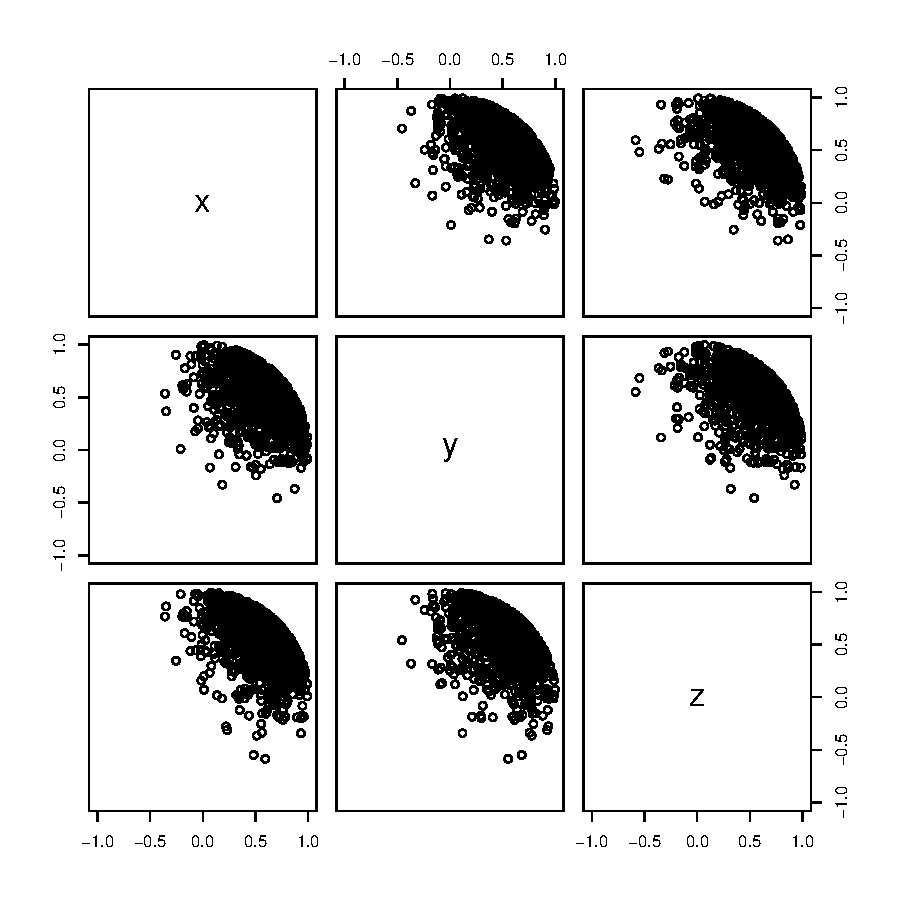
\includegraphics[width=1\textwidth]{sphere_vmf.pdf}
%\caption{Constrained independent Gaussian distribution}
%\end{subfigure}
%%\begin{subfigure}[b]{0.30\textwidth}
%%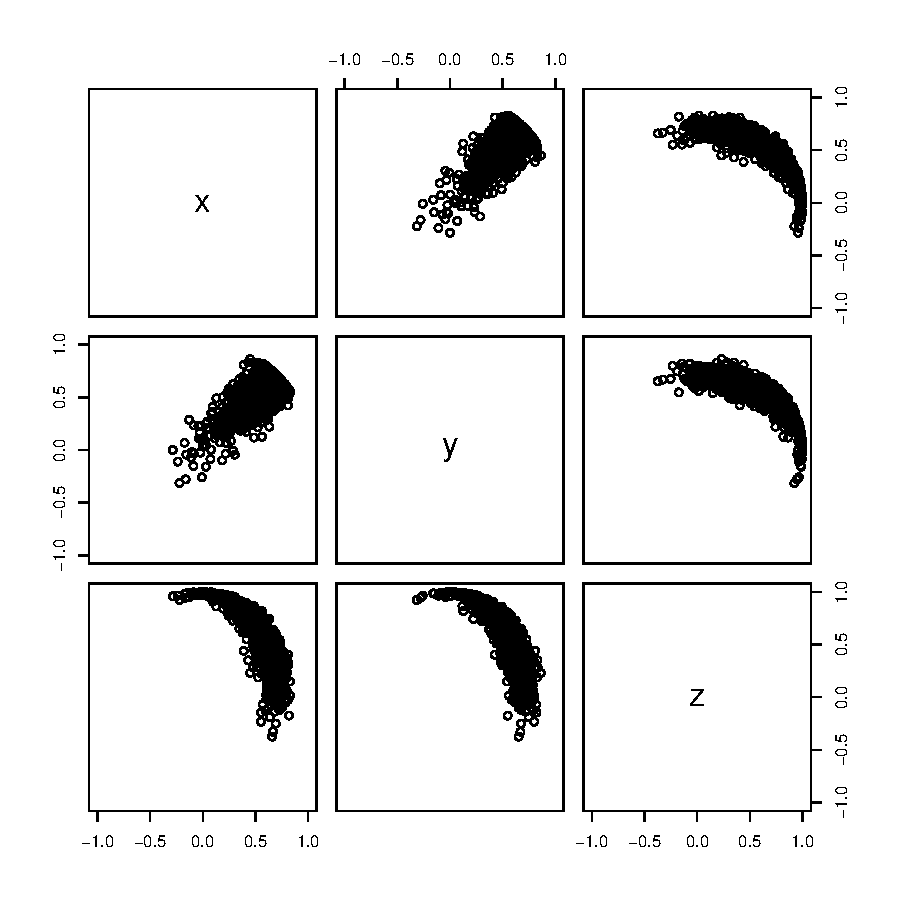
\includegraphics[width=1\textwidth]{sphere_fb}
%%\caption{Constrained correlated Gaussian distribution}
%%\end{subfigure}
%\begin{subfigure}[b]{0.45\textwidth}
%%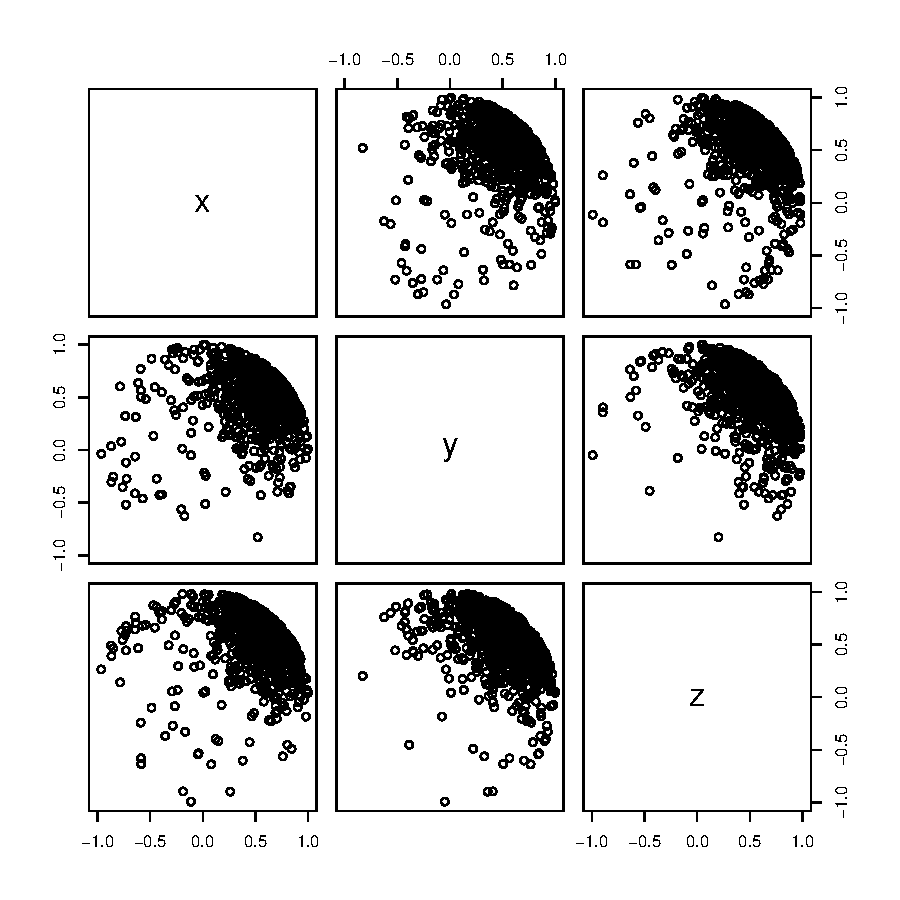
\includegraphics[width=1\textwidth]{sphere_t}
%\caption{Constrained independent $t_3$ distribution}
%\end{subfigure}
%\caption{Sectional view of random samples from constrained distributions on a unit sphere inside $\bb R^3$. The distributions are derived through conditioning on $\theta'\theta=1$ based on unconstrained densities of (a) $\No( F, \diag\{0.1\})$, 
%%(b) $\No(F, \left[\protect\begin{smallmatrix} 0.1 & 0.09 & 0 \\ 0.09 & 0.1 & 0 \\ 0 & 0 &0.1  \protect\end{smallmatrix}\right])$,
% (b) $t_3(F,\diag\{0.1\} )$, where $F=[1/\sqrt{3},1/\sqrt{3},1/\sqrt{3}]'$\\
%}
%\label{sphere_examples}
%\end{figure}
%
%
%
%\subsection{ Constraint Relaxation for Posterior Inference}
%
%The conditional distribution \eqref{constrainedDensity} allows one to adapt
%simple unconstrained $\pi_{\mc R}(\theta)$ into constrained space. When it
%is used as a prior,
%with  the likelihood as $ L(y;\theta)$  and $y$ the data, one can obtain posterior:
%\be
%\label{exactPosterior}
%\pi(\theta\mid y) & \propto L(y;\theta)\pi_{\mc D}(\theta) \\
%& \propto L(y;\theta) \pi_{\mc
%R}(\theta) /J(v(\theta))\mathbbm{1}_{\theta\in \mc D}.
%\ee
%Clearly, the
%posterior also has support only inside $\mc D$ as well due to the inheritance of
%$\mathbbm{1}_{\theta\in \mc D}$ from $\pi_{\mc D}(\theta)$. On the hand,
%the indicator is often inconvenient for posterior inference. We now develop
% two different strategies to relax the parameter $\theta\in \mc D$ into the neighborhood
%of $\mc D$, obtaining posterior $\theta^*$. Then we directly use $\theta^*$ as approximation
%or project $\theta^*$ back to $\mc D$ for exact inference. We refer this
%strategy as {\bf COnstraint RElaxation (CORE)}.
%
%
% \subsubsection{Approximation CORE}
%
%We first present a general approximation strategy. By putting positive mass around $v(\theta)=\bf
%0$, and let it decay exponentially, we relax the support of $\theta$ into a
%neighborhood surrounding $\mc D $. This generate approximate posterior sample $\theta^*\in \mc R$ via
%
%\be
%\label{approximatePosterior}
%\tilde{\pi}(\theta^*\mid y)  & = \frac{1}{m(\lambda)} L(y;\theta^*) \pi_{\mc
%R}(\theta^*) /J(v(\theta^*)) \exp (- \sum_{k=1}^K |v_k(\theta^*)|^\alpha/\lambda_k),
%\ee
%where $v_k$ is the $k$th equation in $v(\theta)$, $\alpha$ is
%typically chosen as $1$ or $2$ to mimic Laplace or Gaussian kernel, $m(\lambda)$ is a normalizing
%constant such that $\int_{\mc R} \tilde{\pi}(\theta^*\mid y) d\theta^*=1$;
% $\lambda_k\ge 0$ is a
%tuning parameter controling the concentration around $v(\theta^*)=\bf 0$.
%When $\lambda_k=0$ for all $k$, 
%\eqref{approximatePosterior} becomes exact; using small $\lambda_k>0$, \eqref{approximatePosterior}
% conventional Monte Carlo approach can be exploited directly in $\mc R$.
%
%We use a toy example with closed-form posterior to illustrate the  approximation. Consider a posterior from a sum-constrained
%bivariate Gaussian random vector $[\theta_1,\theta_2]' \mid y \sim \No(0,I)
%\mathbbm{1}_{\theta_1+\theta_2-1=0}$. Using
%$v(\theta)=\theta_1+\theta_2-1=0$, $J(v(\theta))=\sqrt 2$, the exact posterior \eqref{exactPosterior} is proportional to 
%$$
%\phi(\theta_1)
%\phi(\theta_2)\mathbbm{1}_{v(\theta)=0}
%$$
%where $\phi(.)$ is the standard
%normal density. The exact posterior density has closed-form
%
%$$
%\pi(\theta\mid y)=\frac{\sqrt{2}}{\sqrt{2\pi}} \exp(-\frac{(\theta_1-\frac{1}{2})^2}{2/2})
%\mathbbm{1}_{\theta_2=1-\theta_1}
%$$
%corresponding to $\theta_1\mid (\theta_1+ \theta_2=1) \sim
%\No(1/2,1/2)$, $\theta_2\mid \theta_1 \sim \delta_{1-\theta_1}(.)$, where
%$\delta$ denotes a point mass. Marginally, it is a degenerate Gaussian:
%$$\begin{bmatrix} \theta_1 \\ \theta_2 \end{bmatrix} \sim
%\No_{\text d} \left(
%\begin{bmatrix} \frac{1}{2} \\ \frac{1}{2} \end{bmatrix},
%\begin{bmatrix} \frac{1}{2} & -\frac{1}{2}  \\  -\frac{1}{2}  & \frac{1}{2} \end{bmatrix}
%\right).$$
%
%Using $ \exp( - (\theta^*_1+\theta^*_2-1)^2/\lambda)$ to
%replace $\mathbbm{1}_{v(\theta)=0}$, we obtain approximation $\theta^*_1 \sim \No(\frac{2}{\lambda+4},\frac{\lambda+2}{\lambda+4})$, $\theta^*_2\mid \theta^*_1 \sim \No(\frac{2}{\lambda+2}(1-\theta^*_1),\frac{\lambda}{\lambda+2})$. Marginally, 
%
%$$\begin{bmatrix} \theta^*_1 \\ \theta^*_2 \end{bmatrix} \sim
%\No \left(
%\begin{bmatrix} \frac{2}{\lambda+4} \\ \frac{2}{\lambda+4} \end{bmatrix},
%\begin{bmatrix} \frac{\lambda+2}{\lambda+4} & -\frac{2}{\lambda+4}  \\  -\frac{2}{\lambda+4}  &\frac{\lambda+2}{\lambda+4} \end{bmatrix}
%\right).$$
%As approximation, one can sample from the non-degenerate distribution using small $\lambda$. Clearly, the approximation error decreases as $\lambda$ gets
%smaller, and intuitively becomes exact when $\lambda\rightarrow 0$. We will formalize
%this notion in the theory section.
%
%\subsubsection{Data Augmentation CORE}
%
%The previous strategy is generally applicable for approximating the indicator
%function. In some less general but
%still common cases, one can relax the parameter $\theta$ to $\theta^*$ through some relaxing function
%$g$ first, if there is an inverse function $g^{-1}$ to project it back to
%$\mc D$, we can use $\theta=g^{-1}(\theta^*)$ to directly reparameterize $\pi_{\mc D}(\theta\mid y)$.
%
%
%The relaxation $\theta^*=g(\theta;w)$ often requires an auxillary parameter
%$w$ that controls the amount of relaxation. Usually $w$ is independent of $\theta$, but can be dependent on $\theta^*$. Treating $w$ as a latent variable from $\pi(w)$  with $\int_{\mc W} \pi(w) dw =1$ and $\mc W$ as
%its support, one uses $g^{-1}(\theta^*;w)$ to reparameterize the exact posterior $\pi_{\mc D}(\theta\mid y)$.
%Standard variable transformation yields new parameterization
%
%
%\be
%\label{reparameterization}
%\pi(\theta^*,w\mid y) & =\pi_{\mc D}(g^{-1}(\theta^*;w)\mid y) \frac{1}{J(g(\theta;w))}  \pi(w) \\
%&\propto \frac{\pi_{\mc R}(g^{-1}(\theta^*;w)\mid y) }{ J(v(\theta))\mid_{\theta=g^{-1}(\theta^*;w)} } \frac{1}{J(g(\theta;w))} \pi(w) 
%\ee
%where   $J(g(\theta;w))$ is the Jacobian of $g$ with respect to $\theta$.
%The indicator function $\mathbbm{1}_{\theta\in \mc D}$ disappears since $g^{-1}(\theta^*;w)\in \mc
%D$ always holds. It can be verified that transforming $\theta^*=g(\theta;w)$  yields $\pi_{\mc D}(\theta\mid y) \pi(w)$, which is the exact posterior augmented
%with latent variable $w$. Therefore, we refer this strategy as data augmentation
%constraint relaxation (DA-CORE). Using DA-CORE, one can directly sample $\theta^*$ and $w$ in less constrained
%space, and apply $\theta=g^{-1}(\theta^*;w)$ in the end to obtain the $\theta$-marginal.
%
%One simple example of relaxation would be scaling of $\theta$ under  norm constraint. For example, in $(p-1)$-simplex,
%$\|\theta\|_1=\sum_{i=1}^p\theta_1=1$ with $\theta\in \mc R=[0,\infty]^p$, one
%can augment an independent latent variable $w\in [0,\infty)$ have
%$\theta_i^*=\theta_i w$, and the inverse $\theta_i=\theta_i^*/w$ with
%$w=\sum_{i=1}^p \theta^*_i$. Suppose exact posterior is a Dirichlet distribution 
%$\theta\mid y\sim \text{Dir}(\alpha)$
%, 
%$$
%\pi_{\mc D}(\theta \mid y)\propto \prod_{i=1}^p \theta_i^{\alpha-1}\mathbbm{1}_{\sum_{i=1}^p\theta_i=1},$$
%then the relaxed parameterization is $$
%\pi(\theta^*,w\mid y) =\pi(\theta^*\mid y)\propto  \prod_{i=1}^{p-1} (\frac{\theta_i^*}{w})^{\alpha-1}  w^{-(p-1)} \pi(w), \quad w=\sum_{i=1}^p \theta^*_i, \quad \theta^*\in(0,\infty)^p.$$
%
%More generally, one can often choose the relaxation $g$ based on the projection $g^{-1}$ that produces $\theta\in \mc D$. To illustrate, we consider the random variable
%$\theta$, a $n$-by-$k$ matrix in the Stiefel manifold $\theta\in \mc V(n,k)=\{\theta\in \bb R^{n\times
%k}: \theta'\theta=I\}$, where $n\ge k$. The QR-decomposition produces such
%an orthonormal matrix, for which a $n$-by-$k$ matrix $X=QR$,
%with $Q\in \mc V(n,k)$ and $R$ $k$-by-$k$ upper triangular and diagonal positive;
% the
%QR decomposition is unique if $X$ is of rank $k$ \citep{gulliksson1992modifying}, which allows us to
%use it as $g^{-1}$. Letting $w$ be a random matrix, $k$-by-$k$, upper triangular and diagonal positive, we have $\theta^*=\theta w$, with $\theta^*$ in rank
%$k$. Suppose $\theta$ is $n$-by-$k$ and from the Matrix Bingham--von Mises--Fisher distribution
%\citep{hoff2009simulation},
%$$\pi_{\mc D}(\theta\mid y)\propto \text{etr}(C'\theta+B\theta'A\theta)  \mathbbm{1}_{\theta'\theta=I_k}$$
%where $\text{etr}$ represents the exponential of trace, $A$ is symmetric $n$-by-$n$, $B$ is symmetric $k$-by-$k$ and $C$ is $n$-by-$k$. The relaxed
%parameterization is
%
%$$\pi(\theta^*, w\mid y) =\pi(\theta^*\mid y)\propto \text{etr}(C'\theta^*w^{-1}+B(\theta^*w^{-1})'A\theta^*w^{-1} \text{det}^{-1}(w), \quad \text{rank}(\theta^*)=k, \quad w= \text{QR.R}(\theta^*)$$
%where $\text{QR.R}$ denotes the function that outputs $R$ matrix in QR decomposition.
%
%In comparison, in other reparameterization such as coordinate system, one can only use equal or less parameters to satisfy the constraint, which can
%be  constringent. In DA-CORE, it is generally
%more flexible with more parameters, thanks to the data augmentation. Since $w$ is a redundant latent variable, one can
%assign $\pi(w)$ to allow greater relaxation, which is commonly associated
%with better performance in posterior sampling. More will be illustrated in
%the simulation.
%
%
% \subsection{Theoretic Properties}
%
%We now present the properties of the proposed approach. We first establish
%that the conditioning approach yields valid probability measure.
%
%We focus on $\mc R$ being a $p$-dimensional Euclidean space and the
%intrinsic dimension of $\mc D$, $\mbox{dim}(\mc D)=s\le p$  is integer.
%Although the
%$p$-dimensional Lebesgue measure can have $\mu^p(\mc D)=0$, it is still possible to define a conditional probability given the event ${v(\theta)=\bf 0}$. We utilize the concept of {\it regular
%conditional probability} (r.c.p.)
%\citep{kolmogorov1950foundations}. For this article to be self-contained,
%we list the definition as below (a more complete review can be found in \cite{leao2004regular}).
%
%Let $(X, \mathscr A, \mu)$ be a probability space and $(Y, \mathscr B)$ a measurable space. A function $v$ is measurable if $v:X\rightarrow Y$, $v^{-1}(\mathscr B)\in \mathscr A$.
%A r.c.p is a function
%$f: Y\times \mathscr A \rightarrow[0,1]$ satisfying:
%
%\begin{enumerate}
%        \item $f(y, .)$ is a measure on $(X,\mathscr A)$ for each $y \in
%        Y$;
%        \item $f(., E)$ is a measurable function on $(Y,\mathscr B)$ for each $E\in \mathscr A$;
%        \item For each $E \in \mathscr A$, $F\in \mathscr B$,
%        $\mu(E \cap v^{-1}(F))=\int_{F} f(y, E) \mu_y(dy)$, with
%        $\mu_y$ the induced measure on $(Y,\mathscr B)$.
%\end{enumerate}
%
%Using the previous notation, we write $f(y,E)= P(\theta\in E\mid
%v(\theta)=y)=\int_E \pi_{\mc R}(\theta
%\mid v(\theta)=y) d\theta$
%
%\begin{remark}
%Assuming $J(v(\theta))> 0$ and there is a finite and
%non-negative integer $s$ such
%that, for some $y\in Y$,
%\be
%m^{s}(y)=\int \frac{\pi_{\mc
%R}(\theta)
%\mathbbm{1}_{v({\theta})=y}}{J(v(\theta))}\mu^s(d\theta)\in(0,\infty),
%\ee
%then
%\begin{equation}
%P(E\mid v(\theta)=y)=\left\{\begin{array}{ll}  \frac{1}{m_s(y)}\int_{E } \frac{\pi_{\mc
%R}(\theta) \mathbbm{1}_{v({\theta})=y}}{J(v(\theta))}\mu^s(d\theta)
%& \text{  , if }m_s(y)\in(0,\infty) \\
%\delta_{x^*}(E) \text{ with fixed } x^*\in \bb R^p
%& \text{  , if }m_s(y)\in\{0,\infty\} \\
%\end{array}\right.
%\end{equation}
%is a valid r.c.p..
%\end{remark}
%\begin{proof} The first two crieria for r.c.p are trivally satisfied. We
%use the Hausdorff measure, the standard tool for geometric measure theory \citep{federer2014geometric}, defined as $\mc H^{s}(A)= \underset{\delta\rightarrow 0}\lim \inf \{ \sum \left[{\text{diam}(S_i)}\right]^s: {A\subseteq \cup S_i, \text{diam}(S_i)\le \delta}, \text{diam}(S_i)=\sup_{x,y\in S}\|x-y\|\}$. We denote the normalized Hausdorff measure as $\bar{\mc H}^{s}(A) =\frac{\Gamma(\frac{1}{2})^{s}}{2^s \Gamma(\frac{s}{2}+1)} \mc H^{s}(A)$. When $s$ is an integer, Lebesgue and normalized Hausdorff measures coincide  $\mu^{s}(A)= \bar{\mc H}^{s}(A)$ \citep{evans2015measure}.
%
%Similar to the proof of (2) of Proposition 2 of \cite{diaconis2013manifold}, using co-area formula \citep{federer2014geometric}:
%
%\be
%\mu^{p}(E\cap v^{-1}(F))= & \int \mathbbm{1}_{\theta \in E} \mathbbm{1}_{\theta \in v^{-1}(F)}\pi_{\mc R}(\theta)\mu^p(d\theta) \\
%= & \int \left[ \int_{v^{-1}(y)} \mathbbm{1}_{\theta \in E} \mathbbm{1}_{v(\theta) \in F}  \frac{ \pi_{\mc R}(\theta)}{J(v(\theta))} \bar{\mc H}^{s}(d\theta)\right] \mu^{p-s}(dy) \\
%= & \int_{F} \left [ \int_{ E}  \frac{ \pi_{\mc R}(\theta) \mathbbm{1}_{v(\theta)=y}}{J(v(\theta))} \mu^{s}(d\theta)  \right] \mu^{p-s}(dy) \\
%\ee
%
%
%For $y\in \{y':m(y')=0\}$, $\int_{ E}  \frac{ \pi_{\mc R}(\theta) \mathbbm{1}_{v(\theta)=y}}{J(v(\theta))} \mu^s(d\theta) \le \int_{ \bb R^{s}}  \frac{ \pi_{\mc R}(\theta) \mathbbm{1}_{v(\theta)=y}}{J(v(\theta))} \mu^s(d\theta) =0$; for $y\in \{y':m(y')=\infty\}$, since $\mu ^{p}(\bb R^p)=\int \mathbbm{1}_{m(y)=\infty}m(y) dy + \int  \mathbbm{1}_{m(y)<\infty}m(y)  dy=1$, one must have $\int \mathbbm{1}_{m(y)=\infty} dy=0$. Combining parts yields
%\be
%\mu(E\cap v^{-1}(F)) & = \int_{F} \mathbbm{1}_{m(y)\in (0,\infty)}\left[
%\int_{E} \frac{\pi_{\mc
%R}(\theta) \mathbbm{1}_{v({\theta})=y}}{J(v(\theta))}
%\mu^{s}(d\theta) \right] \mu^{p-s}(dy) \\
%& = \int_{F} \mathbbm{1}_{m(y)\in (0,\infty)}
%\left[ \int_{E}  \frac{1}{m(y)}  \frac{\pi_{\mc
%R}(\theta) \mathbbm{1}_{v({\theta})=y}}{J(v(\theta))}
%\mu^{s}(d\theta) \right ]  m(y)\mu^{p-s}(dy)\\
%& =\int_F f(y,E) \mu_y(dy) 
%\ee
%
%\end{proof}
%
%The above remark gives the definition of r.c.p given all $v(\theta)\in Y$. It is possible $m^s(y)=0$ or $\infty$ for some $y\in Y$, but as long as  $m^{s}({\bf 0})\in (0,\infty)$ at certain integer $s$, we would have a valid constrained density 
%
%\be 
%\pi_{\mc D}(\theta)=
%\frac{1}{m^{s}({\bf 0})}  \frac{\pi_{\mc
%R}(\theta) \mathbbm{1}_{v({\theta})={\bf 0}}}{J(v(\theta))}
%\ee 
%
%The dimension $s$ is often referred as `intrinsic' dimension of $\mc D$. Formally, one would use a standard concept in geometric measure theory named Hausdorff measure,  \citep{federer2014geometric}. The $d$-dimensional Hausdorff measure is the limit total volume of the $d$-dimenional balls covering $A$, $\mc H^{d}(A)= \underset{\delta\rightarrow 0}\lim \inf \{ \sum \left[{\text{diam}(S_i)}\right]^d: {A\subseteq \cup S_i, \text{diam}(S_i)\le \delta}, \text{diam}(S_i)=\sup_{x,y\in S}\|x-y\|\}$. Then the intrinsic dimension is equal to Hausdorff dimension $s=\inf_{d\ge 0}\{H^d(\mc D)=0\}=\sup_{d\ge 0}\{H^d(\mc D)=\infty\}$, at which the Hausdorff measure transitions from $0$ to $\infty$. Although finding $s$ can be challenging \citep{mardia1975statistics,bowen1979hausdorff}, one could could heuristically test $s\in \{p,p-1,\ldots, 0\}$ if $s$ is known to be an integer. Fortunately, for posterior estimation, there is no need for estimating $s$ or the normalizing constant $m^{s}(\bf 0)$ in Monte Carlo sampling.
%
%We now quantify the approximation error of the approximation CORE \eqref{approximatePosterior}. 
%We use $\Pi(.)$ and $\tilde\Pi(.)$ to represent the measures under exact and approximating distributions. 
% For easier notation, we re-parameterize the approximating part as $\exp(-\lambda^{-1}  v(\theta))$ where $\lambda=\max_k \lambda_k$ and $v(\theta)=\sum_{k=1}^d\frac{|v_k(\theta)|^{\alpha}}{\lambda^*_k}$ with $\lambda^*_k=\lambda_k/\lambda$ and define a conditional expectation, $\mathbb{E}(g(\theta) \mid v(\theta)=x)=  \int_{\bb R^s } \frac{ g(\theta) \mathbbm{1}_{v(\theta)=x} \pi_{\mc R}(\theta)}{ J v(\theta) } d \theta.$
%
% We now assess the behavior of approximation error in terms of 1-Wasserstein distance, as $\lambda$ decreases towards $0$. The 1-Wasserstein distance $W_1(\Pi,\tilde\Pi)$ represents the minimal amount of transport needed to transform one distribution to another. Formally, it is defined as
%
%$$W_1(\Pi,\tilde\Pi)=\underset{\gamma\in \Gamma(\Pi,\tilde\Pi)}{\inf}\int \|\theta-\theta^*\| d\gamma(\theta,\theta^*)$$ 
%where $\Gamma(\Pi,\tilde\Pi)$ is the family of all joint measures of with $\Pi$ and $\tilde\Pi$ as the marginals, and $\|\theta-\theta^*\|$ is the
%Euclidean distance.
%
%
%
%%Due to similar form in prior and posterior, we now introduce some general notation. Let $\pi_{\mc R}(\theta)$ be the normalized density in $\mc R$ such that $\int \pi_{\mc R}(\theta)=1$, which is $\pi_{0,\mc R}(\theta)$ for prior and $L(y;\theta)\pi_{0,\mc R}(\theta)$ for posterior;% Suppose $\Phi:\mathbb R^p \rightarrow \mathbb R^d$ with $p>d$ is Lipschitz, then the co-area formula \citep{federer2014geometric} is,
%% \begin{equation}
%% \ \int_{\mathbb{R}^n}  f(\theta)J_N\Phi(\theta)\mu^n(d \theta)
%% =\ \int_{\mathbb{R}^m}  \int_{\Phi^{-1}(y)}f(\theta) \mc H^{n-m}(d\theta)\mu^m(d y),
%% \end{equation}
%% where $\mu^k(d\theta)$ a $k$-dimensional Lebesgue measure. 
%
%
%\begin{remark}
%The 1-Wasserstein distance between the measures based on \eqref{exactPosterior} and \eqref{approximatePosterior} has
%$$ \underset{\lambda \rightarrow 0}\lim W_1(\Pi,\tilde\Pi)=0.$$
%Further, for $\alpha=1$ in \eqref{approximatePosterior},
%
%\begin{equation}
%\begin{aligned}
%W_1(\Pi,\tilde\Pi) \le \lambda (\frac{k_1 k_2}{m(0)^2} + \frac{k_1}{m(0)}) + \exp(- \lambda^{-1} t )(\frac{k_1}{m(0)^2} + \frac{k_3}{m(0)}),
%\end{aligned}
%\end{equation}
%where $k_1=\underset{g:\|g\|_L\le 1}\sup\underset{t^*\in [0,t)}\sup \|\mathbb{E}(g(\theta^*) \mid v(\theta^*)=t^*)\|$, $k_2= \underset{t^*\in (0,t)}\sup  m(t^{*})$ and $k_3=\underset{g:\|g\|_L\le 1} \sup \mathbb{E}(\| g(\theta )\|)$.
%\end{remark}
%
%
%\begin{proof}[Proof]
%Let $g:\mathbb{R}^p\rightarrow \mathbb{R}$ be a 1-Lipschitz continuous function, i.e. $\|g-g(y)\|\le \|x-y\|$, denoted by $\|g\|_L\le 1$. 
%By Kantorovich-Rubinstein duality, the 1-Wasserstein distance based on Euclidean metric equals to: 
%
%\begin{equation}
%W_1(\Pi,\tilde\Pi)=\underset{g:\|g\|_L\le 1}\sup \int g \Pi(dx) -  \int g(y) \tilde\Pi(dy) 
%\end{equation}
%
%Taking $g(\theta)=\exp(-\lambda^{-1}v(\theta))$ in the co-area formula yields
%\begin{equation}
%\begin{aligned}
%m_\lambda
%& = \int_\mathbb{R}  \left[ \int_{v^{-1}} \frac{ \exp(- \lambda^{-1} v(\theta) ) \pi_{\mc R}(\theta)}{ J v(\theta) }  \bar{\mc H}^{p-d}(d \theta) \right] \mathbbm{1}_{x \ge 0}  d x \\
%& = \int_\mathbb{R}  m\exp(- \lambda^{-1} x ) \mathbbm{1}_{x \ge 0}  d x .
%\end{aligned}
%\end{equation}
%
%Taking $g(\theta)={\mathbbm{1}_{v(\theta)=0}}$ yields 
%\begin{equation}
%m_0
%= \int_\mathbb{R} \left[ \int_{v^{-1}(y)} \frac{ \pi_{\mc R}(\theta) }{ J v(\theta) }  \bar{\mc H}^{p-d}(d \theta) \right]\mathbbm{1}_{y=0} dy   =  \int_{v^{-1}(0)} \frac{ \pi_{\mc R}(\theta) }{ J v(\theta) } \bar{\mc H}^{p-d}(d \theta) =m(0)
%\end{equation}
%
%
%Clearly $m_\lambda \ge m_0$.
%
%1. Asymptotic result:
%
%We have
%
%\begin{equation}                
%\label{wass0}
%\begin{aligned}
%&\underset{g:\|g\|_L\le 1}\sup\int g(\theta)  \left[ \frac{ \exp(- \lambda^{-1} v(\theta)) } {  m_\lambda}  - 
%\frac{ \mathbbm{1}_{v(\theta)=0} } {  m_0} 
%\right]  \frac{\pi_{\mc R}(\theta)}{Jv(\theta)}  \bar{\mc H}^{p-d}(d \theta) \\
%&= \underset{g:\|g\|_L\le 1}\sup\int_\mathbb{R}  \mathbb{E}(g(\theta) \mid x)  \left[ \frac{ \exp(- \lambda^{-1} x) \mathbbm{1}_{x \ge 0}} {  m_\lambda}  - 
%\frac{ \mathbbm{1}_{x=0} } {  m_0} 
%\right] d x \\
%&=      \underset{g:\|g\|_L\le 1}\sup\int_\mathbb{R}  \mathbb{E}(g(\theta) \mid x)  \left[ \frac{  1} {  m_\lambda}  - 
%\frac{ 1 } {  m_0} 
%\right]\mathbbm{1}_{x=0} d x  + \underset{g:\|g\|_L\le 1}\sup\int_\mathbb{R}  \mathbb{E}(g(\theta) \mid x)\frac{ \exp(- \lambda^{-1} x)} {  m_\lambda}  
%\mathbbm{1}_{x > 0} d x \\
%& \le \underset{g:\|g\|_L\le 1}\sup \|\mathbb{E}(g(\theta) \mid 0)\| \left[ \frac{ 1 } {  m_0} -\frac{  1} {  m_\lambda}   
%\right] + \frac{1} {  m_0} \underset{g:\|g\|_L\le 1}\sup \int_\mathbb{R}  \|\mathbb{E}(g(\theta) \mid x)\| { \exp(- \lambda^{-1} x)}
%\mathbbm{1}_{x > 0} d x \\      
%\end{aligned}
%\end{equation}
%
%
%Note $m_\lambda\le \int_\mathbb{R} m \mathbbm{1}_{x \ge 0}  dx =\int_\mathbb{R} \pi_{\mc R}(\theta) =1$. By dominated convergence theorem, 
%
%\begin{equation}
%\lim_{\lambda\rightarrow 0}m_\lambda= \int_\mathbb{R}  m \lim_{\lambda\rightarrow 0}\exp(- \lambda^{-1} x ) \mathbbm{1}_{x \ge 0}  d x = m_0.
%\end{equation}
%
%
%Since 
%$ \underset{g:\|g\|_L\le 1}\sup \int_\mathbb{R}  \|\mathbb{E}(g(\theta) \mid x)\| { \exp(- \lambda^{-1} x)} dx \le \int_\mathbb{R} \underset{g:\|g\|_L\le 1}\sup \|\mathbb{E}(g(\theta) \mid x)\| { \exp(- \lambda^{-1} x)} dx$,
%letting $q_\lambda=       \underset{g:\|g\|_L\le 1}\sup \|\mathbb{E}(g(\theta) \mid x)\| { \exp(- \lambda^{-1} x)}
%\mathbbm{1}_{x > 0}  $, we have $0\le q_1-q_{\lambda_1}\le q_1-q_{\lambda_2}$ for $1\ge\lambda_1\ge \lambda_2$, by monotone convergence theorem, $\lim_{\lambda\rightarrow 0}\int [ q_1-q_\lambda]dx = \int [q_1- q_0 ]dx$ hence $\lim_{\lambda\rightarrow 0}\int q_\lambdadx =0$. Combining the results yields 
%
%
%
%\begin{equation}
%\underset{\lambda \rightarrow 0}\lim W_1(\Pi,\tilde\Pi)=0.        \end{equation}
%
%2. Non-asymptotic result:
%
%
%\begin{equation}
%\label{wass1}
%\begin{aligned}
%\frac{1}{m_0}-\frac{1}{m_\lambda} & \le  \frac{   \int_\mathbb{R}  m \exp(- \lambda^{-1} x ) \mathbbm{1}_{x > 0}  d x } {  m_0^2}  \\
%&= \frac{1}{ m_0^2} \left[ \int_0^{t}  m \exp(- \lambda^{-1} x ) dx + \int_t^{\infty}  m \exp(- \lambda^{-1} x ) dx \right] \\
%&\le \frac{1}{ m_0^2} \left[  \underset{t^*\in (0,t)}\sup m(t^{*})\int_0^{t} \exp(- \lambda^{-1} x ) dx + \exp(- \lambda^{-1} t )\int_t^{\infty}  m dx  \right] \\
%&\le \frac{1}{ m_0^2} \left[\lambda \underset{t^*\in (0,t)}\sup  m(t^{*})  + \exp(- \lambda^{-1} t ) \right] 
%\end{aligned}
%\end{equation}
%
%\begin{equation}
%\label{wass2}
%\begin{aligned}
%& \underset{g:\|g\|_L\le 1}\sup\int_\mathbb{R}  \|\mathbb{E}(g(\theta) \mid x)\| { \exp(- \lambda^{-1} x)}  \mathbbm{1}_{x > 0} d x \\
%&\le \underset{g:\|g\|_L\le 1}\sup\underset{t^*\in (0,t)}\sup \|\mathbb{E}(g(\theta) \mid t^*)\|     
%\int_0^{t} \exp(- \lambda^{-1} x ) dx + \exp(- \lambda^{-1} t ) \underset{g:\|g\|_L\le 1}\sup \int_t^{\infty}   \|\mathbb{E}( g(\theta )\mid x)\| dx \\
%&\le \underset{g:\|g\|_L\le 1}\sup\underset{t^*\in (0,t)}\sup \|\mathbb{E}(g(\theta) \mid t^*)\|     \lambda + \exp(- \lambda^{-1} t ) \underset{g:\|g\|_L\le 1} \sup \mathbb{E}(\| g(\theta )\|) \\
%\end{aligned}
%\end{equation}
%
%Combining \eqref{wass0}\eqref{wass1}\eqref{wass2}, $k_1=\underset{g:\|g\|_L\le 1}\sup\underset{t^*\in [0,t)}\sup \|\mathbb{E}(g(\theta) \mid t^*)\|$, $k_2=\underset{g:\|g\|_L\le 1} \sup \mathbb{E}(\| g(\theta )\|)$, $k_3= \underset{t^*\in (0,t)}\sup  m(t^{*})$
%
%
%\begin{equation}
%\begin{aligned}
%& \underset{g:\|g\|_L\le 1}\sup \int g \Pi(dx) -  \int g \tilde\Pi(dx) \\
%        %&\le  \frac{k_1}{ m_0^2} \left[\lambda k_3  + \exp(- \lambda^{-1} t ) \right] 
%        %+ \frac{1} {  m_0} [ k_1       \lambda + \exp(- \lambda^{-1} t )k_2 ]\\     
%        & \le \lambda (\frac{k_1 k_3}{m_0^2} + \frac{k_1}{m_0}) + \exp(- \lambda^{-1} t )(\frac{k_1}{m_0^2} + \frac{k_2}{m_0})
%        \end{aligned}
%        \end{equation}
%
%
%        \end{proof}
%
%        
%
%
%The first part shows the asymptotic accuracy of the approximation. The second part shows the rate with non-asymptotic $\lambda$ under mild assumptions. The interpretation for these assumptions is that if in a small space expansion of $\mc D$, defined as $\{\theta^*: v(\theta^*)\in [0,t] \}$, the marginal density of $v(\theta^*)$ and the conditional expectation of Lipschitz functions are bounded $k_1,k_2= \mc O(1)$, and the expected norm of Lipschitz function are smaller than a bound that grows near exponentially $k_3 = \mc O(\lambda \exp(t/\lambda))$, then the distance $W_1(\Pi,\tilde\Pi)$ converges to $0$ in $\mc O(\lambda)$ as $\lambda\rightarrow 0$.

\alex{
\section{Constrained Relaxation Methodology}
Suppose $\theta$ is an $\mathcal{R}$-valued random variable with $\dim(\mathcal{R})=r<\infty$ and that $\theta$ is subject to some constraints which restrict it to a subset $\mathcal{D} \subset \mathcal{R}$. In the Bayesian setting, of principle interest here, $\theta$ is a parameter which is known to satisfy some constraints such that it resides in $\mathcal{D}$.  In this case, a common approach is to choose a prior distribution with support $\mathcal{D}.$ However, aside from some special cases, a suitable choice of prior may be limited.
 \leo{In my opinion, constructing/choosing prior for constrained space
is a separate issue, which does not involve  `relaxation', so perhaps we
can have a short section before and motivated for more computational stuffs.  }
  Moreover, sampling $\theta$ from the constrained space, when possible, may be difficult or computationally intractable.

One potential strategy to alleviate this issue is to construct an approximate distribution which places a high probability on $\mathcal{D}$ but has support in $\mathcal{R}$ by `relaxing' the constraints.   As a motivating example, consider the case where $\theta$ has density $\pi_\mathcal{R}(\theta)$ with support $\mathcal{R}$ and $\mathcal{D}$ is a measureable subset with positive measure.  The posterior density of $\theta$ given data $Y$ and $\theta \in \mathcal{D}$ is, $$\pi(\theta | \theta \in \mathcal{D}, Y) \propto \mathcal{L}(\theta; Y) \pi_\mathcal{R}(\theta) \mathbbm{1}_\mathcal{D} (\theta)$$ with likelihood function $\mathcal{L}(\theta;Y)$, and data $Y$. 
As an approximation, suppose we used the density 
\begin{equation}
\label{EQ:Rel_Dens_Motivation}
\tilde{\pi}(\theta) \propto \mathcal{L}(\theta; Y)  \pi_\mathcal{R}(\theta) \exp\bigg(-\frac{1}{\lambda} v_\mathcal{D}(\theta)\bigg)
\end{equation} where $v_\mathcal{D}(\theta) = \inf_{x\in\mathcal{D}} ||\theta-x||$ is a measure of the distance from $\theta$ to the constrained space for some metric $||\cdot||$. 

Note that $\mathbbm{1}_\mathcal{D}(\theta)$ is the pointwise limit of $\exp\big(- \nu_\mathcal{D}(\theta)/\lambda)$ (except perhaps on the boundary of $\mathcal{D}$) as $\lambda \to 0^+.$ However, (1) has support $\mathcal{R}$ for all $\lambda > 0$, hence `relaxing' the constraint.   Since (1) is supported on $\mathcal{R}$ it is more suitable for off-the-shelf MCMC sampling strategies.   Ideally, one would hope that samples from (1) could be easily generated and that they would behave as if drawn from the fully conditioned distribution when $\lambda$ is sufficiently small. We consider this approach when adapted to a number of settings, but generally we refer to it as constraint relaxation (\core).

These observations motivate a number of questions about \core\, which we investigate in the article.  (i) For what types of distributions and constraints is CORE suitable? (ii) Is there a general approach for constructing the `relaxed' constraint? (iii) How well do samples from the relaxed constraint represent those from the fully conditioned distribution? (iv) How does the approximation depend on the tuning parameter $\lambda$? 

The answers to (ii) - (iv) depend largely upon (i).  Therefore, beginning with (i), we assume $\theta$ is a continuous random variable (e.g. $\mathcal{R}$ is $\mathcal{R}$, $[0,\infty)^d$, $\mathbb{R}^{n\times k}$) and $\theta$ has an unconstrained prior density $\pi_\mathcal{R}(\theta)$ which is absolutely continuous with respect to Lebesque measure on $\mathcal{R}$ hereby denoted as $\mu_\mathcal{R}$.  We investigate two general types of constraints. 



First, we consider the simpler case where $\mathcal{D}$ has positive measure, i.e. $\int_\mathcal{D} \pi(\theta) \mu_\mathcal{R}(d\theta) >0.$ \leo{Generally,} Inequality constraints (e.g. $a_i < \theta_i < b_i$, $a^T\theta < 0$, $||\theta||_2^2 < 1$) fall into this category. The analysis in this case will be more straightforward as we can follow traditional approaches to conditional probability. Here, the construction of the relaxed constraint will follow the form of Eq. (\ref{EQ:Rel_Dens_Motivation}).

Secondly, we consider the case where $\mathcal{D}$ is a measure zero subset of $\mathcal{R}$. In particular, we restrict ourselves to the setting where $\mathcal{D}$ can be represented implicitly as the solution set of a consistent system of equations $\{\nu_i(\theta) = 0\}_{i=1}^s$ so that $\mathcal{D} =\{\theta | v_j(\theta) =0, \, j = 1, \dots,s\}$ is a co-dimension $s$ submanifold of $\mathcal{R}$.  For a given constrained space, $\mathcal{D}$, there may be multiple choices of the constraints $v_i$. However, there are technical requirements, discussed in Section \ref{SEC:Zero_measure_theory}, which limit the potential choice of the constraint questions \leo{perhaps avoid cross-referencing
later section, by simplifying this sentence
to `There are some limitations on the types of constraint one could use,
however we note that ...'}. 

While these criteria may seem restrictive, we note that many common constraints (e.g. $||\theta||^2 = 1$, $\sum_i \theta_i = 1$, $\theta \in V_k(\mathbb{R}^n)$ where $V_k(\mathbb{R}^n$) is the Stiefel manifold) fall into this category.  In this case, the conditional distribution of $\theta$ given $\theta \in \mathcal{D}$, must be handled with care since $\int_D \pi_R(\theta) d\mu_\mathcal{R} (\theta) =0$.  However, the requirement that $\mathcal{D}$ has codimension $s$ will serve two purposes.  First, it will make the construction of conditional distributions on $\mathcal{D}$ using the tools of geometric measure theory more intuitive.  Secondly, it will motivate a general strategy for choosing appropriate constraint equations and in constructing a relaxed density similar to (1). 

Prior to discussing rigorous details on the use of \core, we first review the  principle details of the method in the context of a few examples.  These examples were chosen to highlight the basic strategy of implementing \core\, and to clarify some of the main ideas behind the supporting theory.


%The remainder of this section is organized as follows.  In 2.1, we briefly discuss the construction of the fully constrained distribution $\theta|\theta \in \mathcal{D}$ when $\mathcal{D}$ is measure zero \leo{based on density
%proportional to $\mathcal{L}(\theta; Y)  \pi_\mathcal{R}(\theta)$}.  Additionally, we suggest a general strategy for choosing the relaxed density.  Relevant theorems comparing the relaxed and fully constrained distributions are given. In Section 2.2, we consider the simpler case where $\mathcal{D}$ has positive measure.  Again, we suggest a general strategy for constructing the relaxed density and supply relevant theorems.  For clarity, proofs of the theorems contained in 2.1 and 2.2 are supplied in the appendix. In Section 2.3, we discuss a number of examples which highlight the methods from 2.1 and 2.2.
%

\subsection{Positive measure constrained spaces}
\label{SEC:Positive_measure_methods}
In this subsection, we consider the case where $\mathcal{D}$ has positive measure.  As such, the constrained posterior density, $\pi_\mathcal{D},$ for $\theta|\theta \in \mathcal{D}$ and data $Y$ is 

$$\pi_\mathcal{D}(\theta|Y) = \frac{\mathcal{L}(\theta; Y) \pi_\mathcal{R}(\theta)\mathbbm{1}_\mathcal{D}(\theta)}{\int_\mathcal{D} \mathcal{L}(\theta; Y) \pi_\mathcal{R}(\theta)d\mu_\mathcal{R}(\theta)}\propto \mathcal{L}(\theta; Y) \pi_\mathcal{R}(\theta)\mathbbm{1}_\mathcal{D}(\theta). $$
This constrained density is absolutely continuous with respect to $\mu_\mathcal{R}$.  

Suppose we approximate $\pi_\mathcal{D}$ with a relaxed density $$\tilde{\pi}_\lambda(\theta) = \mathcal{L}(\theta; Y) \frac{\mathcal{L}(\theta; Y)\pi_\mathcal{R}(\theta)\exp\big(-\frac{v_d(\theta)}{\lambda}\big)}{\int_{\mathcal{R}}\mathcal{L}(\theta; Y) \pi_\mathcal{R}(\theta)\exp\big(-\frac{v_d(\theta)}{\lambda}\big) d\mu_\mathcal{R}(\theta)} \propto \mathcal{L}(\theta; Y) \pi_\mathcal{R}(\theta)\exp\big(-\frac{v_d(\theta)}{\lambda}\big)$$
which is also absolutely continuous with respect to $\mu_\mathcal{R}.$
Here $\lambda >0$ and $v_d(\theta)$ is a scalar-valued function which measures the distance from $\theta$ to the constrained space $\mathcal{D}$, i.e. $v_d(\theta) = 0 $ $\forall \theta \in \mathcal{D}$ and is positive otherwise.  Formally, as $\lambda \to 0^+$, $\exp(-v_d(\theta)/\lambda) \to \mathbbm{1}_\mathcal{D}(\theta)$ pointwise.  If $\mathcal{D}$ is an open subset of $\mathcal{R}$, this limit may not hold on the boundary of $\mathcal{D}$, denoted $\partial \mathcal{D}$.  However, in general $\mu_\mathcal{R}(\partial \mathcal{D}) = 0$ and we are working with densities. Thus, we can ignore this issue.

There are many possible choices for $v_d$ which may be selected for different reasons.  Perhaps the simplest choice is to take
\begin{equation}
\label{EQ:Isotrophic_relaxation}
v_d(z) =  \inf_{x\in\mathcal{D}} ||z-x||_k
\end{equation}
where $||\cdot||_k$ denotes the distance using the $k$-norm. Under this choice of $v_d$, the relaxation is isotrophic. More generally, one could use
\begin{equation}
v_d(z) = \inf_{x\in\mathcal{D}} \sqrt{(x-z)^T A (x-z)}\label{EQ:anistrophic_relaxation}
\end{equation} for some positive definite matrix $A$. In this case, the relaxation is anistrophic, and can be viewed as a form of directional relaxation. This choice of distance, $v_d$, allows for a more detailed specification of the rates at which individual components of $\theta$ relax to $\mathcal{D}$.  In fact, if one seeks to constrain $\theta$ within a neighborhood containing $\mathcal{D}$, the matrix $A$ can be chosen to preferentially relax the constraint and limit deviations from $\mathcal{D}$ in certain directions.

So long as $v_d(\theta)$ is zero for $\theta \in \mathcal{D}$ and positive for $\theta\in\mathcal{D}^c$, it follows that $\pi_\mathcal{D}$ is the pointwise limit of $\tilde{\pi}$ for $\mu_\mathcal{R}$ a.e. $\theta$ in $\mathcal{R}.$  It is natural to expect that estimates of $E[g(\theta)|\theta\in\mathcal{D}]$ can be obtained by using the relaxed posterior density, $\tilde{\pi}_\lambda$, rather than the fully constrained posterior density $\pi_\mathcal{D}$. For small $\lambda$, we anticipate
$$\int_\mathcal{R} g(\theta)\tilde{\pi}_\lambda(\theta) d\mu_\mathcal{R}(\theta) \approx \int_\mathcal{D} g(\theta)\pi_\mathcal{D}(\theta) d\mu_\mathcal{R}(\theta) .$$
Rigorous details for the validity of this approximation, a suitable class of functions for which it applies, and rates of convergence in $\lambda$ are contained in Section \ref{SEC:Positive_measure_theory}. For now, we discuss the implementation in the case of a bivariate normal distribution constrained to the region below a line in the $\theta_1-\theta_2$ plane.

\subsubsection{Example: Gaussian  under Linear Inequality}


Suppose that $\theta = (\theta_1,\theta)$ follows a bivariate Gaussian with mean $\mu \in\mathbb{R}^2$ and covariance matrix, $\Sigma = \sigma^2 I_2$, $\sigma > 0$. Furthermore, suppose $\theta$ is constrained to the triangular region $\mathcal{D} = \{(\theta_1,\theta_2) | \, \theta_1+\theta_2\le 1, \theta_1\ge0, \theta_2 \ge 0\}.$ Let $$v_d(\theta_1,\theta_2) = \max(\theta_1+\theta_2 -1,0) + \max(-\theta_1,0) + \max(-\theta_2,0).$$
Then, $v_d(\theta_1,\theta_2) = 0$ $\forall \theta\in\mathcal{D}$. Otherwise, $v_d$ is positive.  The fully constrained density of $\theta$ given that $\theta\in \mathcal{D}$ is then,
$$\pi_\mathcal{D}(\theta_1,\theta_2)= \pi(\theta_1,\theta_2|\theta\in\mathcal{D})= \frac{\exp\bigg(-\frac{||\theta||^2}{2\sigma^2}\bigg)\mathbbm{1}_\mathcal{D}(\theta)}{\int_0^1\int_0^{1-\theta_1}\exp\bigg(-\frac{||\theta||^2}{2\sigma^2}\bigg)d\theta_2d\theta_1}\propto \exp\bigg(-\frac{||\theta||^2}{2\sigma^2}\bigg) \mathbbm{1}_{\{\theta_1+\theta_2\le 1\}\cap \{\theta_1 \in [0,\infty)\}\cap \{\theta_2\in[0,\infty)\}} .$$
Alternatively, the relaxed density, $\tilde{\pi}_\lambda(\theta)$, is
\begin{align*}
\tilde{\pi}_\lambda(\theta) &=\frac{\exp\bigg(-\frac{||\theta||^2}{2\sigma^2} - \frac{1}{\lambda}v_d(\theta) \bigg)}{\int_{\mathbb{R}^2} \exp\bigg(-\frac{||\theta||^2}{2\sigma^2}-\frac{1}{\lambda}v_d(\theta) \bigg)d\theta_2d\theta_1}\\
& \propto \exp\bigg(-\frac{||\theta||^2}{2\sigma^2}\bigg)\exp\bigg( - \frac{1}{\lambda}[\max(\theta_1+\theta_2 -1,0) + \max(-\theta_1,0) + \max(-\theta_2,0)] \bigg).
\end{align*}
\subsection{Measure zero constraints}
\label{SEC:Zero_Measure_Methods}


\subsubsection{Example: von Mises--Fisher on Unit Circle}


\section{Analytical Results}
\subsection{Positive measure constrained spaces}
\label{SEC:Positive_measure_theory}

We return now to the case where $\mathcal{D}$ has positive measure with respect to the unconstrained posterior density so $$\int_\mathcal{D} \mathcal{L}(\theta; Y) \pi_\mathcal{R}(\theta)d\mu_\mathcal{R}(\theta) >0.$$ Recall that in this case, the fully constrained posterior distribution is

$$\pi_\mathcal{D}(\theta|Y) = \frac{\mathcal{L}(\theta; Y) \pi_\mathcal{R}(\theta)\mathbbm{1}_\mathcal{D}(\theta)}{\int_\mathcal{D} \mathcal{L}(\theta; Y) \pi_\mathcal{R}(\theta)d\mu_\mathcal{R}(\theta)}\propto \mathcal{L}(\theta; Y) \pi_\mathcal{R}(\theta)\mathbbm{1}_\mathcal{D}(\theta). $$  Whereas, the relaxed posterior density is
$$\tilde{\pi}_\lambda(\theta) = \mathcal{L}(\theta; Y) \frac{\mathcal{L}(\theta; Y)\pi_\mathcal{R}(\theta)\exp\big(-\frac{v_d(\theta)}{\lambda}\big)}{\int_{\mathcal{R}}\mathcal{L}(\theta; Y) \pi_\mathcal{R}(\theta)\exp\big(-\frac{v_d(\theta)}{\lambda}\big) d\mu_\mathcal{R}(\theta)} \propto \mathcal{L}(\theta; Y) \pi_\mathcal{R}(\theta)\exp\big(-\frac{v_d(\theta)}{\lambda}\big)$$
for some distance function $v_d(\theta)$ which is zero for $\theta \in \mathcal{D}$ and positive for $\theta \in (\mathcal{D}^c)^o.$  

Both of these densities are absolutely continuous with respect to Lebesque measure on $\mathcal{R}$.  Thus, the expectation of $g$ given $\theta\in\mathcal{D}$, is
\begin{equation}
\label{EQ:Expectation_Positive_Measure_Constraint}
E[g(\theta)|\theta\in\mathcal{D}] = \int_\mathcal{D} g(\theta)\pi_\mathcal{D}(\theta)d\mu_\mathcal{R} = \frac{\int_\mathcal{D} g(\theta)\mathcal{L}(\theta; Y) \pi_\mathcal{R}(\theta)d\mu_\mathcal{R}(\theta)}{\int_\mathcal{D} \mathcal{L}(\theta; Y) \pi_\mathcal{R}(\theta)d\mu_\mathcal{R}(\theta)}.
\end{equation} 
Similarly, the expected value of $g$ with respect to the relaxed density, denote as $E_{\tilde{\pi}_\lambda}[g]$, is then,
\begin{equation}
\label{EQ:Expectation_Positive_Measure_Relaxed}
E_{\tilde{\pi}_\lambda}[g(\theta)] = \int_\mathcal{R} g(\theta)\tilde{\pi}_\lambda(\theta)d\mu_\mathcal{R} = \frac{\int_\mathcal{R} g(\theta)\mathcal{L}(\theta; Y) \pi_\mathcal{R}(\theta) \exp(-v_d(\theta)/\lambda)d\mu_\mathcal{R}(\theta)}{\int_\mathcal{R} \mathcal{L}(\theta; Y)\exp(-v_d(\theta)/\lambda) \pi_\mathcal{R}(\theta)d\mu_\mathcal{R}(\theta)}.\end{equation}

We can now consider the behavior of $E_{\tilde{\pi}_\lambda}[g]$ as $\lambda \to 0^+.$

\begin{lemma}
\label{THM:positive_measure_approximation_error}
Suppose $g \in \mathbb{L}^1(\mathcal{R}, \mathcal{L}(\theta;Y)\pi_\mathcal{R}d\mu_\mathcal{R})$.  Then,
$$\bigg|E[g(\theta) |\theta\in\mathcal{D}] - E_{\tilde{\pi}_\lambda}[g(\theta)]   \bigg| \le \frac{\int_{\mathcal{R}\setminus \mathcal{D}} (C_\mathcal{R}E|g(\theta)|+|g(\theta)|) \mathcal{L}(\theta; Y) \pi_\mathcal{R}(\theta)\exp(-v_d(\theta)/\lambda ) d\mu_\mathcal{R}(\theta)}{\big[\int_\mathcal{D} \mathcal{L}(\theta; Y) \pi_\mathcal{R}(\theta)d\mu_\mathcal{R}(\theta)\big]^2 }$$
where $E|g(\theta)| \propto \int_\mathcal{R} |g(\theta)| \mathcal{L}(\theta;Y)\pi_\mathcal{R} d\mu_\mathcal{R}(\theta)$ is the expected value of $|g(\theta)|$ with respect to the unconstrained posterior density and $C_\mathcal{R} = \int_\mathcal{R} \mathcal{L}(\theta;Y)\pi_\mathcal{R}(\theta)d\mu_\mathcal{R}(\theta)$ is the normalizing constant of this unconstrained posterior density. Furthermore, if $v_d(\theta)$ is zero for all $\theta\in\mathcal{D}$ and positive for $\theta\in(\mathcal{R}\setminus\mathcal{D})^o$, it follows from the dominated convergence theorem that $$\bigg|E[g(\theta) |\theta\in\mathcal{D}] - E_{\tilde{\pi}_\lambda}[g(\theta)]   \bigg|\to 0 \text{ as } \lambda \to 0^+.$$
\end{lemma}

Thus, one can obtain sufficiently accurate estimates of $E[g|\theta\in\mathcal{D}]$ by sampling from $\tilde{\pi}_\lambda$ when $\lambda$ is sufficiently small.  From a practical standpoint, it is desirable to understand the rate at which $E_{\tilde{\pi}_\lambda}[g(\theta)] $ converges to $E[g(\theta)\in\mathcal{D}]$. This question is addressed in the following theorem.

\begin{theorem}
\label{THM:Positive_measure_convergence_rate}
Suppose $g \in  \mathbb{L}^2(\mathcal{R}, \mathcal{L}(\theta;Y)\pi_\mathcal{R}d\mu_\mathcal{R})$, $v_d(\theta)$ has the form of Eq. (\ref{EQ:Isotrophic_relaxation}) with $k=2$, $\mathcal{D}$ has a piecewise smooth boundary, and that $\mathcal{L}(\theta;Y)\pi_\mathcal{R}(\theta)$ is continuous on a open neighborhood containing $\mathcal{D}$.  Then for $0<\lambda \ll 1,$
$$ \bigg|E[g(\theta) |\theta\in\mathcal{D}] - E_{\tilde{\pi}_\lambda}[g(\theta)]   \bigg| = O(\sqrt{\lambda}).  $$
\end{theorem}
This theorem follows by applying the Cauchy-Schwartz inequality to the term in the numerator of the bound given in Lemma \ref{THM:positive_measure_approximation_error}.  One can attain a bound depending on the surface area of $\mathcal{D}$ when its is bounded.  More generally, if $\mathcal{D}$ is a unbounded subset of $\mathcal{R}$, one can make use of the co-area formula\cite{federer2014geometric, diaconis2013manifold}. The proofs of Lemma \ref{THM:positive_measure_approximation_error} and Theorem \ref{THM:Positive_measure_convergence_rate} are contained in Appendix \ref{APP:Positive_Measure_Convergence_Proofs}.

These results have some important implications both analytically and numerically.  First, in addition to point estimates, $E[\theta|\theta\in\mathcal{D}]$, it is possible to approximate probabilities $P(\theta \in \mathcal{F}|\theta \in \mathcal{D})$ and higher moments, e.g. $E[\Pi_j \theta_j^{k_j} |\theta\in\mathcal{D}]$, so long as these moments exist for the unconstrained density $\pi_\mathcal{R}.$ 

Secondly, these bounds demonstrate that the error in using the relaxed density to approximate $E[g(\theta)|\theta\in\mathcal{D}]$ is proportional to $\sqrt{\lambda} [\int_\mathcal{D}\mathcal{L}(\theta; Y)  \pi_\mathcal{R}(\theta)d\mu_\mathcal{R}(\theta)\big]^{-2}$ although this rate may not be optimal.  In practice, $\lambda$ may need to be very small, particularly in the case where $0<P(\theta\in\mathcal{D})\ll 1.$ Of course, specific details of the scaling of $\bigg|E[g(\theta) |\theta\in\mathcal{D}] - E_{\tilde{\pi}_\lambda}[g(\theta)]   \bigg|$ will depend upon the choice of $\mathcal{D}$ and $v_d(\theta)$. In practice (see Sections 5), we have observed much better convergence rates.

In general, one avenue for mitigating numerical difficulties which may arise when $\lambda \ll 1$ is needed is to use Eq. \ref{EQ:anistrophic_relaxation} to relax the density in directions where accuracy is less important.  Fortunately, both Lemma\ref{THM:positive_measure_approximation_error} and Theorem \ref{THM:Positive_measure_convergence_rate} will still hold when $A$ is positive definite since this corresponds to a simple re-scaling of the parameter space.






\subsection{Measure zero constrained spaces}
\label{SEC:Zero_measure_theory}

\begin{theorem}
\label{THM:RCP_construction}
\alex{We'll need to decide on a choice of notation for this definition: 

Assume that $J(v(\theta)) > 0$ and that for each $z\in\mathbb{R}^s$ there is a finite non-negative integer $p_z$ such that,  $$m^{p_z}(z) = \int_{\mathbb{R}^ {s}} \frac{\mathcal{L}(\theta; Y) \pi_\mathcal{R}(\theta) \mathbbm{1}_{v(\theta)=z}}{J(v(\theta))} d\bar{\mathcal{H}}^{p}(z) \in (0,\infty).$$
Then, for any Borel subset, $E$, of $\mathcal{R}$, it follows that 
$$P(E|v(\theta) = z) = 
\begin{cases}
\frac{1}{m^{p_z}(z)} \int_E \frac{\mathcal{L}(\theta; Y) \pi_\mathcal{R}(\theta) \mathbbm{1}_{v(\theta)=z}}{J(v(\theta))} d\bar{\mathcal{H}}^{p}(z)  & m^s(z)\in (0,\infty)  \\
\delta (E) & m^p(z) \in \{0,\infty\}
\end{cases}$$
is a valid regular conditional probability for $\theta\in\mathcal{D}.$ Here, $\delta (E)=1$ if $0\in E$ and $0$ otherwise. }
\leo{I suggest we use the $r$ and $(r-s)$ for dimensionality as before,
this changes to:\\
Assume that $J(v(\theta)) > 0$ and that there exists $z\in\mathbb{R}^s$  such that,  $$m^{s}(z) = \int_{\mathbb{R}^ {r-s}} \frac{\mathcal{L}(\theta; Y) \pi_\mathcal{R}(\theta) \mathbbm{1}_{v(\theta)=z}}{J(v(\theta))} d\bar{\mathcal{H}}^{(r-s)}(\theta) \in (0,\infty).$$
Then, for any Borel subset, $E$, of $\mathcal{R}$, it follows that 
$$P(E|v(\theta) = z) = 
\begin{cases}
\frac{1}{m^{s}(z)} \int_E \frac{\mathcal{L}(\theta; Y) \pi_\mathcal{R}(\theta) \mathbbm{1}_{v(\theta)=z}}{J(v(\theta))} d\bar{\mathcal{H}}^{(r-s)}(\theta)  & m^s(z)\in (0,\infty)  \\
\delta (E) & m^s(z) \in \{0,\infty\}
\end{cases}$$
is a valid regular conditional probability for $\theta\in\mathcal{D}.$ Here, $\delta (E)=1$ if $0\in E$ and $0$ otherwise. 
}
\end{theorem}


\begin{theorem}
\label{THM:Relaxed_Expectation_Convergence_Measure_Zero}
Let $m:\mathbb{R}^s\to \mathbb{R}$ and $m_g:\mathbb{R}^s\to \mathbb{R}$ be defined as follows
\begin{align*}
m &= \int_{\nu^{-1}} \frac{\pi_\mathcal{H}(\theta) \mathcal{L}(y;\theta)}{J(\nu(\theta))} d\mathcal{R}^{r-s}(\theta) \\
m_g &= \int_{\nu^{-1}} g(\theta)\frac{\pi_\mathcal{H}(\theta) \mathcal{L}(y;\theta)}{J(\nu(\theta))} d\mathcal{R}^{r-s}(\theta).
\end{align*}
Suppose that both $m$ and $m_g$ are continuous on an open interval containing the origin and that \\ $g\in\mathbb{L}^1(\mathcal{R},\pi_R\mathcal{L}(y;\theta)d\mu_\mathcal{R}) \cap\mathbb{L}^1(\mathcal{D},\frac{\pi_R\mathcal{L}(y;\theta)}{J(\nu(\theta))}d\mu_\mathcal{R})$. Then,
$$\bigg|E_{\tilde{\Pi}}[g] - E[g|\theta \in \mathcal{D}]\bigg| \to 0 \text{ as } \lambda\to 0^+.$$
\end{theorem}

\begin{corollary}
In addition to the assumptions of Theorem \ref{THM:Relaxed_Expectation_Convergence_Measure_Zero}, suppose that both $m$ and $m_g$ are differentiable at $0$. Then
$$\bigg|E_{\tilde{\Pi}}[g] - E[g|\theta \in \mathcal{D}] \bigg| = O\bigg(\frac{\lambda}{|\log \lambda|^s}\bigg)$$
as $\lambda \to 0^+.$
\end{corollary}

}
 
\section{Posterior Computation}

Adapting  unconstrained density into space $\mc D$ often disrupts its posterior conjugacy. Since one can now sample the posterior in $\mc R$ using
 CORE, one can exploit conventional sampling tools such as slice sampling, adaptive Metropolis-Hastings and Hamiltonian Monte Carlo (HMC). In this section, we focus on HMC for its easiness to use and good performance in block updating of parameters.

\subsection{Hamiltonian Monte Carlo under Constraint Relaxation}

We provide a brief overview of HMC for continuous $\theta^*$ under constraint relaxation. Discrete extension is possible via recent work of \cite{nishimura2017discontinuous}. For easy notation, we use $q$ to represent $\theta^*$ under approximation-CORE \eqref{approximatePosterior}, and $\{\theta^*, w\}$ under DA-CORE \eqref{reparameterization}.

In order to sample $q$, HMC introduces an auxillary momentum variable $p \sim \No(0, \mass)$. The covariance matrix $\mass$ is referred to as a \textit{mass matrix} and is typically chosen to be the identity or adapted to approximate the inverse covariance of $q$. HMC then sample from the joint target density $\pi(q, p) = \pi(q) \pi(p) \propto \exp (- H(q, p))$ where, in the case of the posterior under relaxation, 


\begin{equation}
\begin{aligned}
H(q, p)& = U(q)+K(p),\\
\text{where } & U(q) = -\log\pi(q),\\
& K(p) = \frac{p'\mass^{-1} p}{2}.
\end{aligned}
\end{equation}
with $\pi(q)$ is the unnormalized density in \eqref{approximatePosterior} or \eqref{reparameterization}. %$L(\theta^*;y)\pi_{0,\mc R}(\theta^*) \exp( - \sum_k\frac{|v_k(\theta^*)|^\alpha}{\lambda_k}) / J(v(\theta^*))$ based on \eqref{approximatePosterior} and $f(q)= L(g(\theta^*;w);y)\pi_{0,\mc R}(g(\theta^*;w))J(g(\theta^*;w)) / J(v(g(\theta^*;w)))$ based on \eqref{reparametrizedPosterior}. 

From the current state $(q^{(0)},p^{(0)})$, HMC generates a proposal for Metropolis-Hastings algorithm by simulating Hamiltonian dynamics, which is defined by a differential equation:

\begin{equation}
\begin{aligned}
\label{hamiltonian}
\frac{\partial q ^{(t)}}{\partial t} & =\frac{\partial H(q, p)}{\partial p} = \mass^{-1}p,\\
\frac{\partial p^{(t)}}{\partial t}& =-\frac{\partial H(q, p)}{\partial q} = -\frac{\partial U(q)}{\partial q}.
\end{aligned}
\end{equation}

The exact solution to \eqref{hamiltonian} is typically intractable but a valid Metropolis proposal can be generated by numerically approximating \eqref{hamiltonian} with a reversible and volume-preserving  integrator \citep{neal2011mcmc}. The standard choice is the \textit{leapfrog} integrator which approximates the evolution $(q^{(t)},p^{(t)}) \to (q^{(t + \dt)},p^{(t + \dt)})$ through the following update equations:

\begin{equation}
\begin{aligned}
\label{leap-frog}
p \leftarrow p - \frac{\dt}{2} \frac{\partial U}{\partial  q },\quad
q \leftarrow  q  + \dt \mass^{-1}p,\quad
p \leftarrow p -  \frac{\dt}{2}  \frac{\partial U}{\partial  q } 
\end{aligned}
\end{equation}
Taking $L$ leapfrog steps from the current state $(q^{(0)},p^{(0)})$ generates a proposal $(q^{*},p^{*}) \approx (q^{(L \dt)},p^{(L \dt)})$, which is accepted with the probability 
$$1\wedge \exp  \left( - H(q^{*},p^{*}) + H(q^{(0)},p^{(0)}))\right)$$


\subsection{Computing Efficiency and Support Expansion}

Since CORE expands the support from $\mc D$ to $\mc
R$, it is useful to study the effect of space expansion on the computing efficiency. In this section, we provide some  quantification of the effects and provide a practical guidance on choosing $\pi(w)$ or $\lambda$ in the
two strategies.


In understanding the computational efficiency of HMC, it is useful to
consider the number of leapfrog steps to be a function of $\dt$ and
set $L = \lfloor \tau / \dt \rfloor$ for a fixed integration
time $\tau > 0$. In this case, the mixing rate of HMC is completely
determined by $\tau$ in the limit $\dt \to 0$ \citep{betancourt17}. In
practice, while a smaller stepsize $\dt$ leads to a more accurate
numerical approximation of Hamiltonian dynamics and hence a higher
acceptance rate, it takes a larger number of leapfrog steps and
gradient evaluations to achieve good mixing. For an optimal
computational efficiency of HMC, therefore, the stepsize $\dt$ should
be chosen only as small as needed to achieve a reasonable acceptance
rate \citep{beskos13, betancourt14}. A critical factor in determining
a reasonable stepsize is the \textit{stability limit} of the leapfrog
integrator \citep{neal2011mcmc}. When $\dt$ exceeds this limit, the
approximation becomes unstable and the acceptance rate drops
dramatically. Below the stability limit, the acceptance rate $a(\dt)$
of HMC increases to 1 quite rapidly as $\dt \to 0$ and in fact
satisfies $a(\dt) = 1 - \mc O(\dt^4)$ \citep{beskos13}.

For simplicity, the following discussions assume the mass matrix $\mass$ is taken to be the identity. Let $\hess_U(q)$ denote the hessian matrix of $U(q) = - \log \pi(q)$ and let $\xi_1(q)$ denotes the first largest eigenvalue of $\hess_U(q)$. While analyzing stability and accuracy of an integrator is highly problem specific, the linear stability analysis and empirical evidences suggest that, for stable approximation of Hamiltonian dynamics by the leapfrog integrator in $\bb R^p$, the condition $\dt < 2\xi_1(\theta)^{-1/2}$ must hold on most regions of the parameter space \citep{hairer06}.
Besides the eigenvalue, if the support of $q$ is a constrained space $\mc Q$, another limiting factor is roughly the shortest distance to the boundary $\eta (\theta; {\mc Q})= \inf_{q'\not\in \mc Q}\|q'-q\|$. If either $\eta (\theta; {\mc Q})$ or $\xi_1(\theta)^{-1/2}$ 
is close to $0$, the upper bound would be too low to obtain efficient computation.
In constrained model, the parameter space $\mc D$ can have very small $\eta(\theta;\mc D)$. Constraint relaxation can reduce this problem via support
expansion. 

For approximation-CORE \eqref{approximatePosterior}, to control approximation
error, one can choose to relax a subset of constringent constraints. Observing  $\mc D=\cap_{k} D_k$,
each approximation $\exp(-\frac{|v_k(\theta^*)|^\alpha}{\lambda_k})$ corresponds to a constrained space $\mc D_k$.  One practical strategy is that, for $\mc D_k$'s with $\eta(\theta;\mc D_k)\approx 0$, one uses moderate $\lambda_k$ to induce some support expansion (denoted by $\lambda_k\ge \zeta$ with $\zeta$ moderately small but not too close to $0$);  for $\mc D_k$'s without this issue, one uses very small $\lambda_k\approx 0$ to almost always uphold the constraint.
The latter was also suggested by \cite{neal2011mcmc} as creating a high `energy wall'. Noting this could create  inaccuracy of HMC near the boundary with $\lambda_k\approx 0$ under fixed step size,  we use random step size $\epsilon$ at each iteration to reduce the error.


The Hessian $\hess_U(q)$ under approximation-CORE is given by
\begin{equation}
\label{eq:hessian_extrinsic}
\hess_U(q) = -\hess_{\log L(y;\theta^*) \pi_{\mc
R}(\theta^*) /J(v(\theta^*)) }(\theta^*)+\sum_k \lambda_k^{-1} \hess_{|v_k|^\alpha}(\theta^*) \mathbbm{1}_{\theta\not\in \mc D_k},
\end{equation}
where the second term $\lambda_k^{-1} \hess_{v_k}(\theta) \mathbbm{1}_{\theta\not\in \mc D_k}$ is $0$ unless $\theta\not\in \mc D_k$. Since the $\lambda^{-1}_k$'s
in the second term often dominate the eigenvalue, hence $\xi^{-1/2}_1(\theta^*)\approx
\underset{\lambda_k\ge \zeta}{\min}\lambda_k^{1/2}$. A trade-off between approximation accuracy and computational efficiency is involved. Fortunately, as quantified above, the approximation error is often $\mc O( \underset{\lambda_k\ge \zeta}{\max}\lambda_k)
$ and decreases faster than the efficiceny cap $\mc O( \underset{\lambda_k\ge \zeta}{\min}\lambda_k^{1/2})$, as $\lambda_k$ decreases.\ In our experiments, we did find changing from $\lambda_{k}=10^{-4}$ to $10^{-5}$ requires approximately $3$ times of computing budget, due the effect on stability
bound.


On the other hand, since DA-CORE \eqref{reparameterization} does not involve such error trade-off, it is preferred when it is applicable. Letting $\mc Q_\theta\subset \mc D$ denote the support for the constrained $\theta\in \mc D$, the reparameterization changes the support to $Q_{\theta^*}=\{g(\theta;w):\theta\in \mc Q\}$. Therefore, one could choose $\pi(w)$ to substantially increase $\eta(\theta^*; Q_{\theta^*})$.
Since the augmented variable $w$ is redundant, DA-CORE can
be considered as one type of parameter expansion  discovered by \cite{liu1999parameter}, who originally
focused on accelerating  Gibbs sampling of probit regression. 
Although for
greater space expansion,  it is possible to use diffuse or even improper prior for $\pi(w)$ on $Q_{\theta^*}$,
 we recommend assigning $\pi(w)$ loosely centered at $w_0:g(\theta;w_0)=\theta$ (corresponding to when $\theta^*=\theta$), which makes $\theta^*$ a mild relaxation of $\theta$. This ensures no substantial change in $\xi^{-1/2}_1(\theta^*)$ in HMC.

\section{Simulations}
In order to compare against existing approaches on computing efficiency and provide empirical evidence
supporting our previous result, we run simulations on several toy examples
 in this section.
   
\subsection{Example: Gaussian  under Linear Inequality}
In this example, we consider a linear model under a system of linear inequality constraints. Although a
recent work proposed a new customized prior with exhibits posterior conjugacy \citep{danaher2012minkowski},
via the \core\, framework, one can make use of a general Gaussian prior. 

Suppose that we wish to sample from a bivariate Gaussian $\theta=(\theta_1,\theta_2) \sim \No \left( \mu, I\sigma^2\right)$ where $\mathcal{D}=\{(\theta_1,\theta_2) |\theta\in(0,1)^2, \, \theta_1+\theta_2<1\}$,
which forms a triangle in the $\theta_1-\theta_2$ plane.  We investigate this example for two different choices of $(\mu,\sigma^2)$. First, let $(\mu, \sigma^2)=([0.3,0.3],1/{10})$  which centers the distribution of $\theta$ near the center of $\mc D$. Secondly,  $(\mu,\sigma^2) = ([0.7,0.3]',1/10^4)$  which induces a  distribution which is concentrated on the boundary of $\mc D$. 

Let $v_d(\theta)=|1-\theta_1+\theta_2|_+ + |-\theta_1|_+ + |-\theta_2|_+ +|1-\theta_1|_+ +|1-\theta_2| $ where $|x|_+ = \max(x,0)$.  Since the triangle has wide support with $\eta(\theta;\mc D)$ away from $0$, small $\lambda=10^{-8}$
 guarantees almost no approximation error. Figure~\ref{linear_inequality} contains plots which show posterior samples and contours of the constrained posterior density. Clearly, the posterior samples are all inside
$\mc D$. To compare, we ran simple rejection sampling with untruncated normal proposal $\No ( \mu, I\sigma^2)$. As expected, it  suffers from a rapidly growing rejection rate from $12\%$ to $51\%$, as $\mu$ moves further away from the center of $\mc D$.

\begin{figure}[H]
\begin{subfigure}[b]{0.45\textwidth}
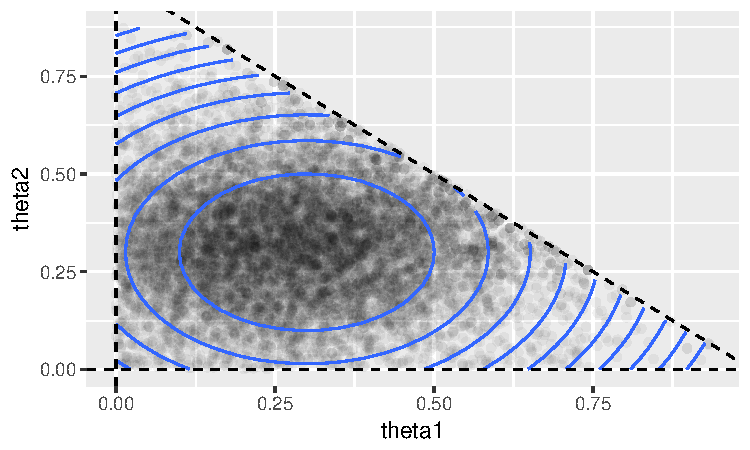
\includegraphics[width=1\textwidth]{linear_inequal_1}
\caption{Constrained $\No([0.3,0.3],1/{10})$}
\end{subfigure}
\begin{subfigure}[b]{0.45\textwidth}
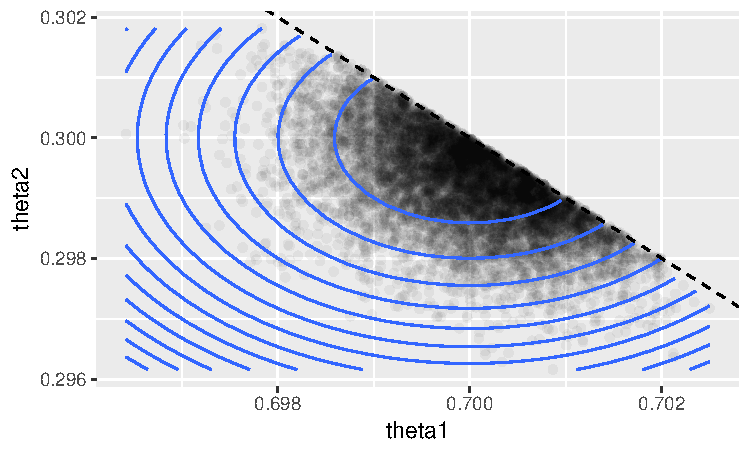
\includegraphics[width=1\textwidth]{linear_inequal_2}
\caption{Constrained $\No([0.7,0.3],1/{10^4})$}
\end{subfigure}
\caption{Posterior sample of bivariate normal distribution subject to linear inequality constraints $\theta\in(0,1)^2,\theta_1+\theta_2<1$, using HMC with  constraint relaxation. Posterior is spread out around the center (panel (a)) or concentrated on the boundary (panel (b)) of the region.}
\label{linear_inequality}
\end{figure}


\subsection{Example: von Mises--Fisher on Unit Circle}
To illustrate equality constraint relaxation, we generate a simple von Mises--Fisher distribution $\pi_{\mc D}(\theta) \propto \exp(F'\theta)$ on a unit circle $\{(\theta_1,\theta_2):\theta_1^2+\theta_2^2=1\}$. We use $F=(5,5)$ to induce a relatively spread-out  $\theta$ on the manifold.
For sampling,
we compare three strategies: approximate-CORE using $\exp(-\frac{|\theta'\theta -1|}{\lambda})$ for approximating the indicator, DA-CORE
using $\theta_1 = \frac{\theta_1^*}{w}, w= \sqrt{(\theta_1^*)^2+ (\theta_2^*)^2}$ and $\pi(w)\sim \No(1,1)\mathbbm{1}_{w>0}$ and  exact  von Mises--Fisher obtained using `movMF' package.

Unlike the previous linear inequality constraint, the unit circle has narrow
$\eta(\theta;\mc D)=0$ for all $\theta\in \mc D$, therefore, some support expansion is needed
for HMC. We test $\lambda = 10^{-3}$, $10^{-4}$ and $10^{-5}$ for approximation-CORE. To compare the efficiency of HMC, we fix the number of leap-frog steps to $20$ within one iteration HMC, and let software STAN
automatically tune for stable step size. Table~\ref{table_circle} shows the effective sample size per $1000$ iterations, the effective `violation' $|v(\theta)|=|\theta_1^{2}+\theta_2^{2}-1|$ and the 1-Wasserstein distance $W_1$ as the approximation error. As $W_1$ is numerically computed, to provide a baseline error, we also calculate the average $W_1$ comparing two independent samples from the same exact distribution. The approximation error $W_1$ based on $\lambda= 10^{-5}$ approximation is indistinguishable from this low numerical error, while the other approximations  have slightly larger error but more effective samples. As expected, the DA-CORE is exact
and has high effective sample size. 
   \begin{table}[H]
   \begin{center}
   \tiny
   \begin{tabular}{ c| c | c| c |c | c}
   \hline     
    & \multicolumn{4}{c|}{ HMC based on CORE}     & Exact  \\   
       \hline     
        & \multicolumn{3}{c|}{Approximation}     & DA-CORE  \\           
       \hline           
     &  $\lambda=10^{-3}$ & $\lambda=10^{-4}$ & $\lambda=10^{-5}$ &  
     &  \\
   \hline
   \hline
   $W_1$ & 0.050 & 0.034  & 0.014 & 0.017  & 0.015 \\

   &  (0.019, 0.095) &(0.027, 0.037) &  (0.013,0.025)  & (0.0012,0.026) & (0.0014,0.025)\\

   \hline
   $|v(\theta)| \mid y$ 
   & $9\times 10^{-4} $ 
   & $9\times 10^{-5} $ 
   & $9\times 10^{-6} $ &0 & 0\\
   & $(2.6 \cdot 10^{-5}, 3.3\cdot 10^{-3})$& $(2.0 \cdot 10^{-6}, 3.4\cdot 10^{-4})$& $(2.7 \cdot 10^{-7}, 3.5\cdot 10^{-5})$&  & \\
   \hline
   ESS /1000 Iterations &  751.48  & 260.54 & 57.10 & 788.30    \\
   \hline  
   \end{tabular}
   \end{center}
   \caption{Benchmark of constraint relaxation methods on sampling von--Mises Fisher distribution on a unit circle. For each approximation CORE, average approximation error (with 95\% credible interval, out of $10$ repeated experiments) is computed, and numeric error of $W_1$ is shown under column `exact' as comparing two independent copies from the exact distribution\label{table_circle}.
Effective sample size shows DA-CORE and approximation-CORE with relatively large $\lambda$ have high computing efficiency.
}
   \end{table}

\subsection{Dirichlet on a Simplex}
Lastly, we experiment with a particularly challenging distribution on a 
$(p-1)$-simplex, defined by $\{\theta: \theta\in(0,\infty)^p,\sum_{i=1}^p \theta_i=1\}$. We consider Dirichlet distribution $\text{Dir}(\alpha)$, with
$\pi_{\mc D}(\theta)\propto \prod_{i=1}^p\theta_i^{\alpha-1}$. When the concentration
parameter $\alpha<1$, $\text{Dir}(\alpha)$ exhibits sparse property that some $\theta_i$'s become very close to $0$, which is exploited in topic modeling \citep{wang2009decoupling} and shrinkage
\citep{bhattacharya2015dirichlet} literature. Despite the simple form, the computation can be quite difficult
 if there is large uncerntainty associated with $\theta$ on top of sparsity.
 The distribution will be multi-modal with distribution scattered along the boundary of the simplex (Figure~\ref{simplex}(a)).

To illustrate, we consider $p=3$ and various values of $\alpha\in \{1,0.5,0.1,0.01\}$. We test the performance of approximation-CORE and DA-CORE. To compare, we also test the standard HMC using coordinate
system $\theta_1=\cos^2(\theta_1^*), \theta_2=\sin^2(\theta_1^*)\cos^2(\theta_2^*), \theta_3=\sin^2(\theta_1^*)\sin^2(\theta_2^*)$ for $\theta^*\in (0,2\pi)^2$,
which is equivalent to stick-breaking representation \citep{ishwaran2001gibbs}; and the geodesic
HMC utilizing the geometric flow directly on the simplex \citep{byrne2013geodesic}.
For all HMCs, we fix the number of steps in each iteration to be $30$ and tune the step size to have  effective sample size as large as possible.

Table~\ref{simplex_tb} lists the effective sample sizes under different $\alpha$'s.
As $\alpha$ becomes smaller than $1$, approximation-CORE and geodesic HMC become worse in performance, while DA-CORE
 and coordinate system are much less impacted.
Figure~\ref{simplex}(b) shows at $\alpha=0.01$, the approximation-CORE and geodesic
HMC are stuck for a long time, while DA-CORE works substantially better. As a well-tested reparameterization,  HMC based on coordinate system still works acceptably well in this case.

The difficulty that approximation-CORE encountered was  anticipated. \cite{byrne2013geodesic} have previously reported similar
slow-down of geodesic HMC computing on hyper-Dirichlet  distribution \citep{hankin2010generalization} with $\alpha<1$. Comparing these two approaches, geodesic HMC relies on restricting the kinetic flow on $\mc D$ via its product with the metric tensor, and approximation-CORE relies
on creating high energy wall in the potential energy. The latter can
be viewed as an approximation
to the former, which explains the similarity in performance.


\begin{figure}[H]
\begin{subfigure}[b]{0.45\textwidth}
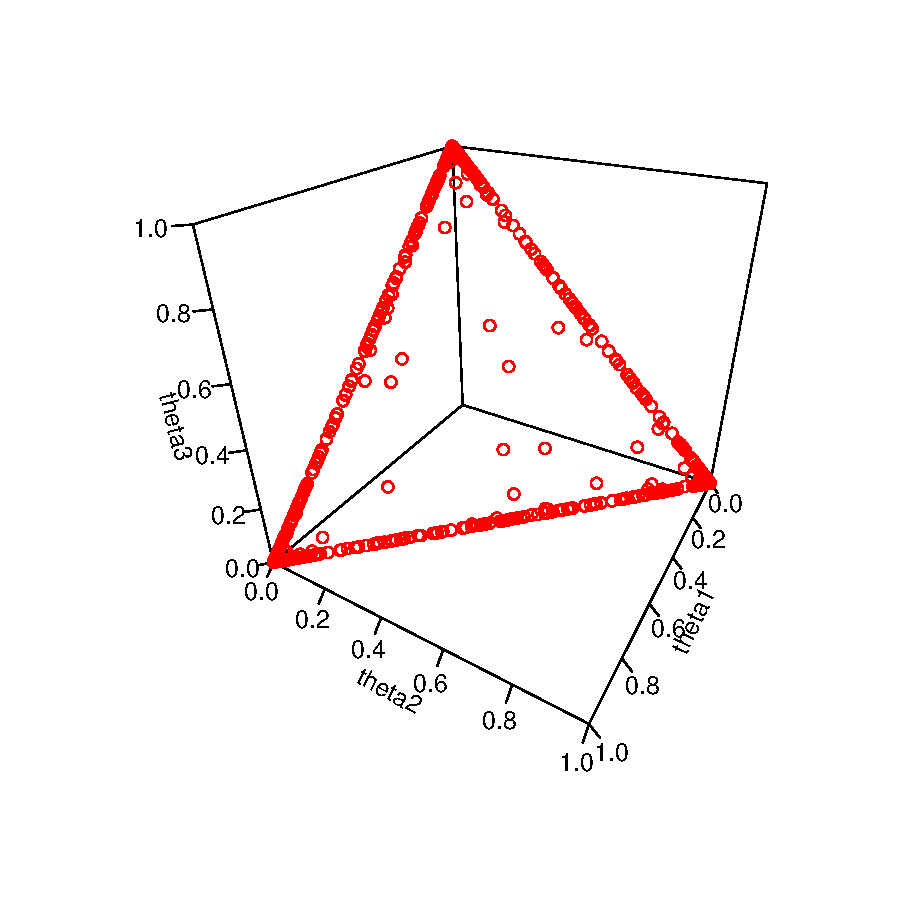
\includegraphics[width=1\textwidth]{simplex001}
\caption{$2,000$ samples from $\text{Dir}(0.01)$ on $2$-simplex.}
\end{subfigure}
\begin{subfigure}[b]{0.45\textwidth}
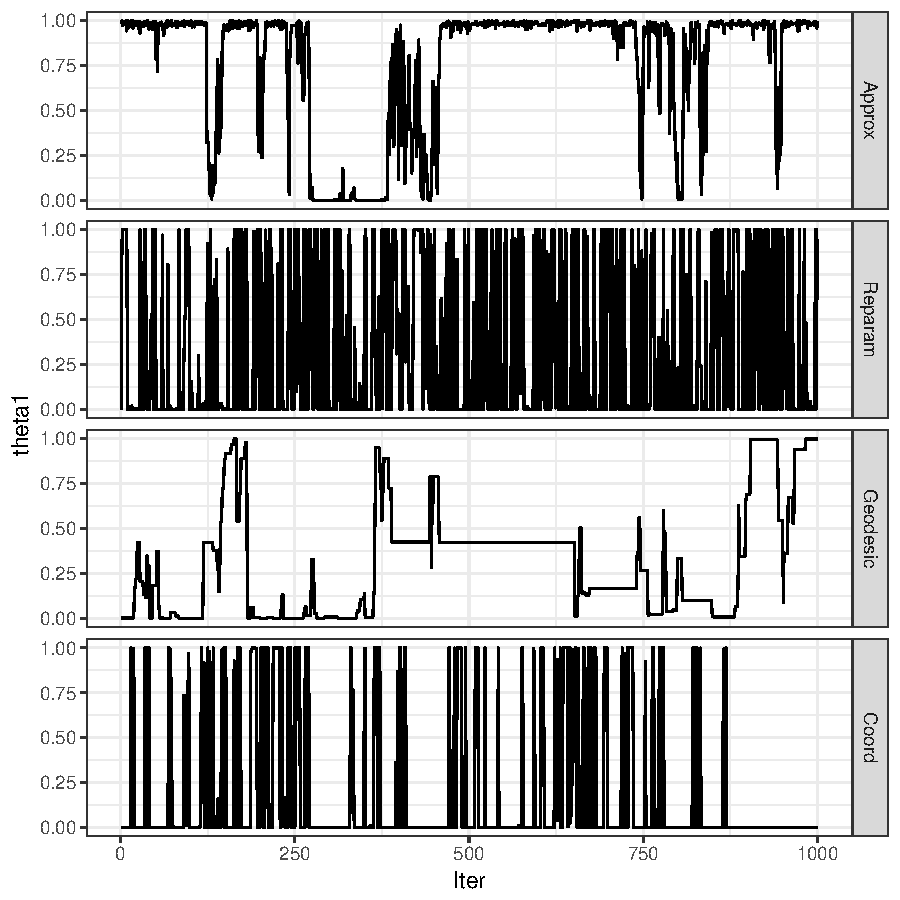
\includegraphics[width=1\textwidth]{simplexTrace001}
\caption{Traceplot of $\theta_1$ using 4 types of HMCs.}
\end{subfigure}
\caption{Sampling of Dirichlet on an simplex with distribution concentrated on the boundaries.
Panel(a) illustrates the distribution under $\text{Dir}(0.01)$; Panel(b)
compares the traceplots of 4 different types of HMCs, which are based on: approximation-CORE with $\lambda=10^{-3}$, DA-CORE, geodesic flow on simplex \citep{byrne2013geodesic} and coordinate
system.}
\label{simplex}
\end{figure}


   \begin{table}[H]
     
   \begin{center}
   \tiny
   \begin{tabular}{ l| r | r| r |r | r}
   \hline     
    & \multicolumn{3}{c|}{HMC based on CORE}     & Geodesic HMC  & Coord
    System HMC \\   
        & {Approx $\lambda=10^{-3}$} & {Approx $\lambda=10^{-4}$}      & DA
        &  \\  \hline         
   ESS /1000 Iter. ($\alpha=1$) & 511.43   & 146.07  & 947.53 &  174.14
   & \bf 961.08     \\
      ESS /1000 Iter. ($\alpha=0.5$) & 145.15  & 33.16  &\bf  912.94  & 31.47  & 846.92   \\
            ESS /1000 Iter. ($\alpha=0.1$) &  88.32   & 26.88& \bf 992.75  &28.70  & 875.83    \\
   ESS /1000 Iter. ($\alpha=0.01$) & 20.54 & 3.91 & {\bf 722.44} & 17.26  & 128.55  \\
   \hline  
   \end{tabular}
   \end{center}
   \caption{Average effective sample size per $1000$ iterations in $\text{Dir}(\alpha)$,
   under different $\alpha$. \label{simplex_tb}
}
   \end{table}

   \section{Application: Finding Sparse Basis in a Population of Networks}

 We now consider a real data application in brain network analysis. 
 The brain connectivity structures are obtained in the data set KKI-42 (Landman et al. 2011), which consists of $n=21$ healthy subjects without any history of neurological disease. We take the first scan out of the scan-rescan data
as the input. Each observation is a $V\times V$ symmetric network, recorded as an adjacency matrix $A_i$ for $i=1,\ldots,n$. The regions are constructed via the Desikan et al. (2006) atlas, for a total of V = 68 nodes.
For the $i$th matrix $A_i$, $A_{i,k,l} \in \{0,1\}$ is the element on the $k$th row and $l$th column of $A_i$, with $A_{(i,k,l)}=1$ indicating there is an connection between $k$th and $l$th region, $A_{(i,k,l)}=0$ if there is no connection. The matrix is symmetric due to the undirectedness of the network,
but the diagonal records $A_{(i,k,k)}$ for all $i$ and $k$ are missing due
to the lack of meaning for self-connectivity. 


One scientific interest in neuroscience is to quantify the variation of brain networks and identify the  regions
(nodes) that contribute to it. Extending 
factor analysis to multiple matrices, one appealing approach
is to have the networks share a common factor matrix but let the  loadings
vary across subjects. This
can be considered as a simplified equivalent of three-way
tensor factorization \citep{kolda2009tensor}. Then to selectively identify the important nodes, one natural way is to apply shrinkage on the elements
of factor matrix.


Geometrically, the factor matrix, denoted by $\{U_1,\ldots,U_d\},$ reside on a Stiefel manifold $\mc V(n,d)=\{U: U'U=I_d\}$, where $U=[U_1,\ldots,U_d]$ is the $n\times d$ matrix. Using $r$ to index $1,\ldots,d$, each frame $U_r$ represents a $(n-1)$-hypersphere. Applying shrinkage forces some of its sub-coordinates to be close to $0$, which
is  reducing each $U_r$ onto a lower-dimensional hypersphere.
Although previous work was done using sparse PCA \citep{zou2006sparse} for
continuous outcome,  little work has been done in a probabilistic model for
binary matrices.

To apply shrinkage in the constrained space, we adopt the induced prior  as common in Bayesian  literature (reviewed by
\cite{polson2012local}), which usually takes the form hierarchical structure $\theta_i\mid
\kappa_i  ,\sigma\sim \No(0,\kappa_i \sigma), \quad \kappa_i\sim G_1, \quad \sigma \sim G_2$ with
$\kappa_i$, $\sigma$ as the local and global scale parameters.  However,
when constraining $\theta_i$, one caveat would be only adapting the conditional density $\No(\theta_i;\kappa_i \sigma)$, which  yields intractable normalizing constant involving $\kappa_i \sigma$ in the conditional. This difficulty can be avoided by
reparameterizing\ $\theta_i=\eta_i\kappa_i\sigma$ with $\eta_i\sim\No(0,1)$, and adapting the {\it joint} density of $\{\eta_i,\kappa_i,\sigma\}$ on constrained
space instead. The
joint density will not have intractable constant as long as the hyper-parameters in $G_1$ and $G_2$ are fixed.

We now
take the Dirichlet-Laplace prior \citep{bhattacharya2015dirichlet} as unconstrained distribution
$\pi_{\mc R}$ and adapt it onto Stiefel manifold via \eqref{constrainedDensity}.
   \begin{equation*}
   \begin{aligned}
   & A_{(i,k,l)} \sim \text{Bern}( \frac{1}{1+ \exp(-\psi_{(i,k,l)}- z_{(k,l)})})\\
   & \psi_{(i,k,l)} = \sum_{r=1}^{d}  v_{(i,r)} u_{(k,r)} u_{(l,r)}  \\
   & U'U=I_{d} \text{ with } U=\{u_{(k,r)}\}_{k=1,\ldots,n; r=1,\ldots,d}\\
           & u_{(k,r)}= \eta_{(k,r)}\kappa_{(k,r)}\sigma_{u} \\
   & \eta_{(k,r)}\sim \text{Lap}(0,1), \quad \{\kappa_{(1,r)}\ldots \kappa_{(V,r)}\} \sim \text{Dir}(\alpha),
    \quad \sigma^2_{u}\sim \text{IG}(2,1)\\   
   & z_{(k,l)} \sim \No(0,\sigma^2_z), \quad  \sigma^2_z \sim \text{IG}(2,1)
   \\
   & v_{(i,r)} \sim \No(0,\sigma^2_{v,(r)}), \quad  \sigma^2_{v,(r)} \sim \text{IG}(2,1)
   \end{aligned}
   \end{equation*}
   for $k>l$, $k=2,\ldots, V$, $i=1,\ldots,n$;  $\text{Lap}(0,1)$ denotes
   the Laplace distribution centered at $0$ with scale $1$; $Z=\{z_{(k,l)}\}_{k=1,\ldots,V;l=1,\ldots,V}$ is a symmetric unstructured matrix that serves as the latent mean; $\{ v_{(i,r)}\}_{r=1,\ldots,d}$
is the loading for the $i$th network, with each $v_{(i,r)}>0$; for all other scale parameters $\sigma^2_.$, we
choose weakly informative prior inverse Gamma $\text{IG}(2,1)$, as appropriate for the scale under the logistic link. To induce sparsity in each Dirichlet,
we use $\alpha=0.1$ as suggested by 
\cite{bhattacharya2015dirichlet}.

 
There are two types of constraints in the model,  $U'U=I_d$ and $\sum_{k=1}^V \kappa_{(k,r)}=1$ for $r=1,\ldots,d$. Taking $v_1(U)= U'U-I_d$ and $v_2(\kappa_{(k,r)})=\sum_{k=1}^V \kappa_{(k,r)}-1$ for each $r$, the Jacobian is  constant in \eqref{constrainedDensity}. For posterior computation, we use DA-CORE
as described above.
Using latent variable $w_U$ $d$-by-$d$ upper triangular and positive diagonal
matrix, and $w_{\kappa,{(r)}}>0$  for $r=1,\ldots ,d$, we relax the parameters
to
$$U^*=U w_U, \quad \kappa^*_{(k,r)}=\kappa_{(k,r)} w_{\kappa,{(r)}},$$
which yields re-parameterization via  projection
\begin{equation}
\begin{aligned}
& U=U^* w_U^{-1}, \quad  w_U=\text{QR.R}(U^*), \\
& \kappa_{(k,r)} = \frac{\kappa^*_{(k,r)}}{w_{\kappa,{(r)}}}, \quad  w_{\kappa,{(r)}}= \sum_{k=1}^V \kappa^*_{(k,r)}\\
& \eta_{k,r}= \frac{u_{(k,r)}}{\kappa_{(k,r)}\sigma_{u}},
\end{aligned}   
\end{equation}where $\text{QR.R}$ denotes the function that outputs $\text{R}$ matrix in
QR decomposition.
To control the amount of relaxation, we assign $w_U$ near $I_d$ via $\pi(w_U)\propto \text{etr}\left[ -\frac{(w_U-I_d)'(w_U-I_d)}{\lambda}\right]$ and $w_{\kappa,{(r)}}$
near $1$ via $\pi(w_{\kappa,{(r)}})\propto \exp\left[ -\frac{(w_{\kappa,{(r)}}-1)^2}{\lambda}\right]$ and set $\lambda=10^{-3}$.


For comparison, we test with the specified model (i) against (ii) the  same
model except with simple $u_{(k,r)}\sim \No (0,\sigma^2_u)$ instead of the shrinkage prior and (iii) the  same
model except  without the orthonormality constraint $U'U=I$ and the shrinkage prior.
We run all models for $10,000$ iterations and discard the first $5,000$ iteration
as burn-in.
For each iteration, we run $300$ leap-frog steps. For efficient computing, we truncated $d=20$. 

Table~\ref{network_model} lists the benchmark results. Compared to (i) and
(ii), the unconstrained model (iii) suffers from very low effective sample
size, due to the serious convergence issue in the factor matrix $U$. As explained
by previous findings in matrix/tensor factorization \citep{hoff2016equivariant},   the factor matrix could
scale and rotate without changing the likelihood,  and  substantial improvement
could be obtained by applying orthonormality constraint.


Figure~\ref{network_model_basis}(a)
plots the posterior mean loadings $v_{(i,r)
}$, with each line representing one subject. For all $i=1,\ldots,21$, the
lines drop quickly to near $0$ after $r\ge 5$ in  model (i)
and (ii), but only do so
until $r\ge 10$ in model (iii). This indicates that independent factors are more effective  representation of the span, compared to non-orthogonal ones. Clearly,
(i) shows more variability than (ii) in the loading $v_{(i,r)}$. We validate these models by calculating area under the receiver operating characteristic curve  (AUC) based on the mean predicted probability and the binary outcome $A_{(i,k,l)}$, using the fitted data and the other unused rescan data from the $21$ subjects.
The models (i) and (ii) with orthonomality constraint perform similarly well, and clearly better than 
the unconstrained model (iii) in prediction AUC.  
 \begin{table}[H]
   \begin{center}
   \tiny
   \begin{tabular}{ l| c | c| c }
   \hline     
 Model   &  (i).with shrinkage \&\ orthonormality    & (ii).with  orthonormality only  & (iii).unconstrained \\         
       \hline           
     Fitted AUC &  97.9\%  & 97.1\%  & 96.9\%     \\
   \hline
     Prediction AUC & 96.2\% & 96.2\%  & 93.6\%      \\
   \hline
   ESS /1000 Iterations &  193.72  & 188.10  & 8.15     \\
   \hline  
   \end{tabular}
   \end{center}
   \caption{Comparing 3 models for 21 brain networks
   \label{network_model}}
   \end{table}

Figure~\ref{network_model_basis}(b) compares the models (i) and (ii) over the top $6$ frames of $U_r$, with  $r$
 re-ordered such that $\sigma^2_{v,(1)}\ge \sigma^2_{v,(2)}\ge \ldots \ge \sigma^2_{v,(d)}$. The posterior of $U_1,U_2,U_3$ look very similar between the two, whereas $U_4,U_5,U_6$ have a considerable subset
of points close to 0 in the model with shrinkage prior.

\begin{figure}[H]
\centering
\begin{subfigure}[b]{0.8\textwidth}
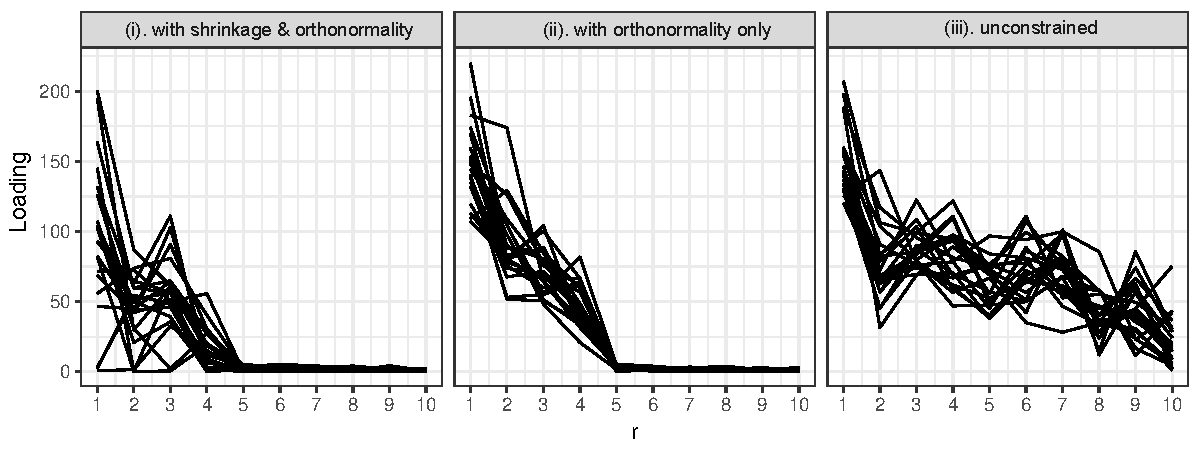
\includegraphics[width=1\textwidth]{network_loading}
\caption{Posterior mean of the loadings $v_{i,r}$ for 21 subjects using three
models. Each line represents the loadings for one subject over $r=1,\ldots10$.}
\end{subfigure}
\begin{subfigure}[b]{1\textwidth}
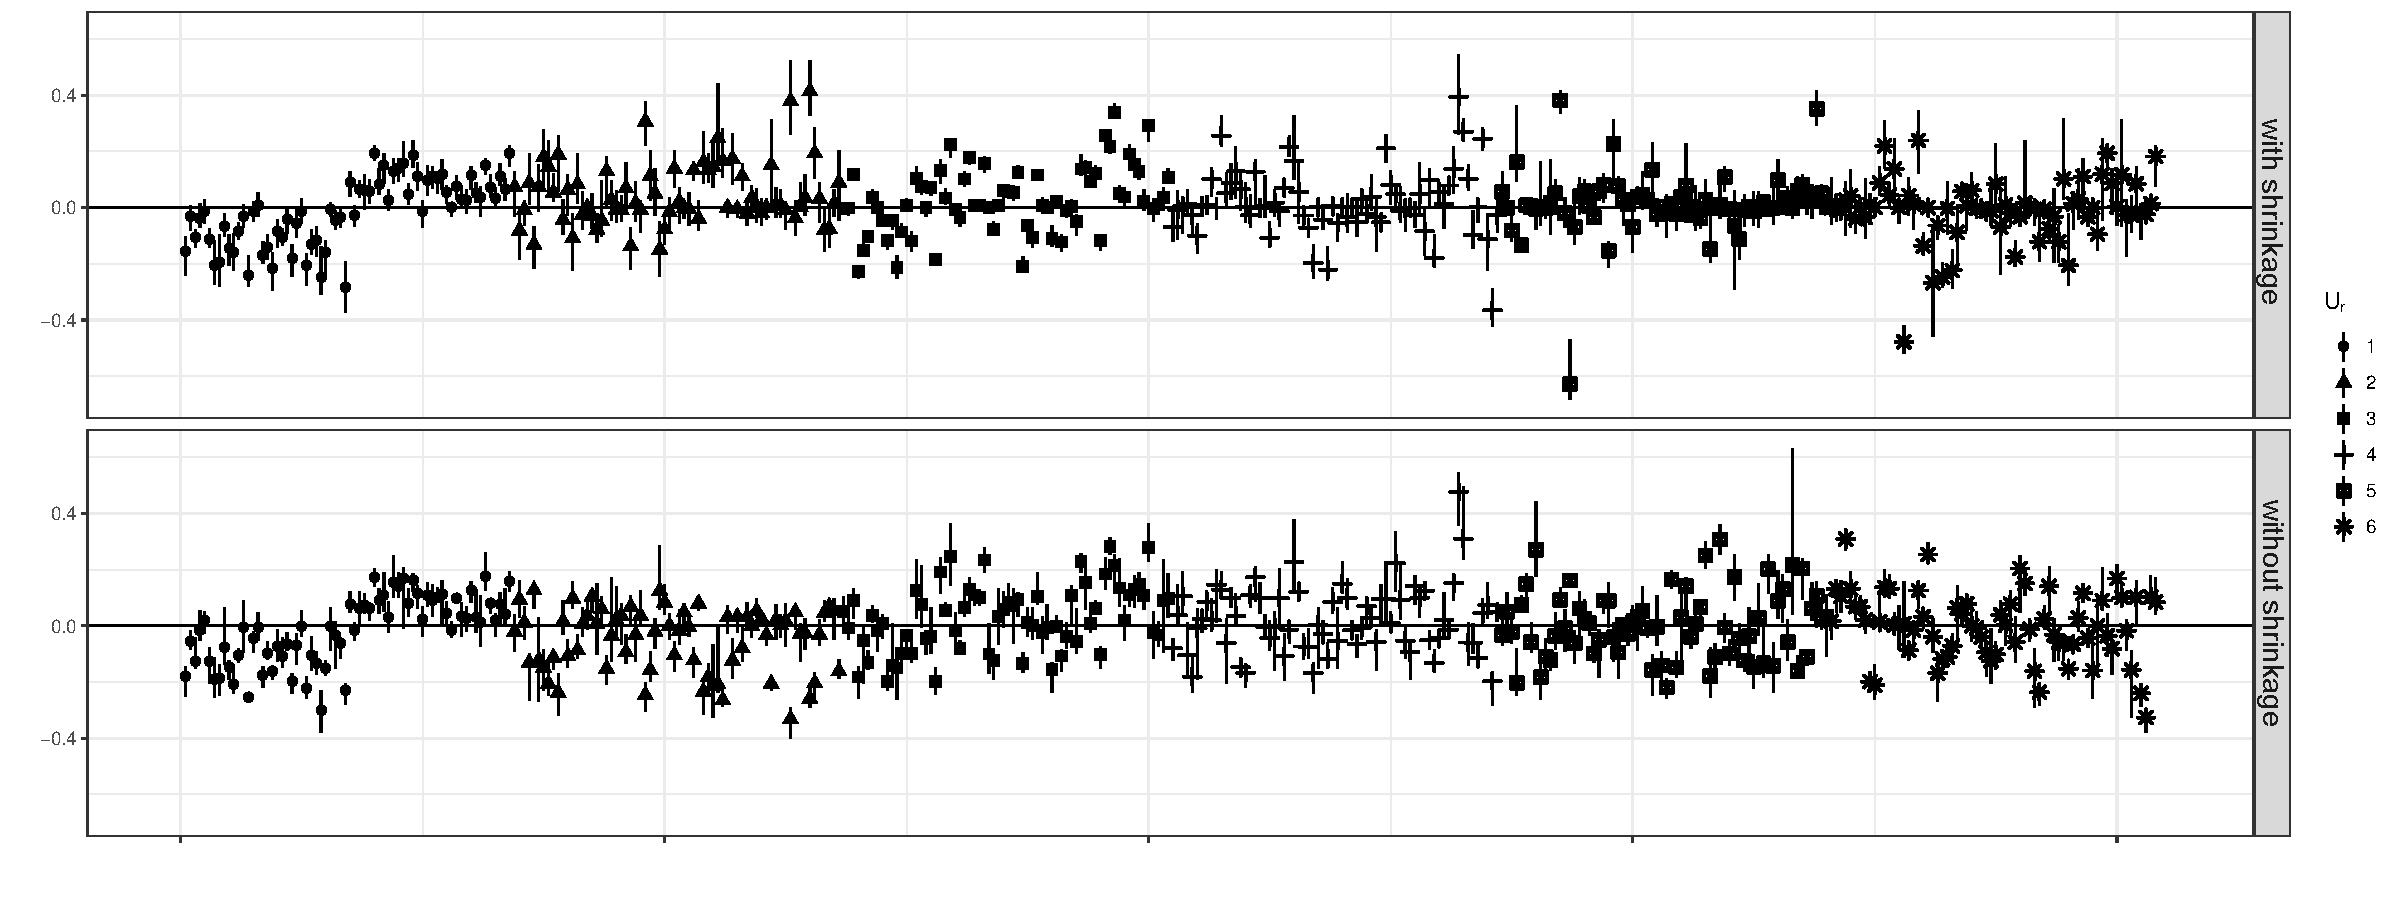
\includegraphics[width=1\textwidth]{network_factor.pdf}
\caption{Posterior mean and pointwise $95\%$ credible interval of  the factors
$U_1,\ldots,
U_6$ in the two constrained models. }
\end{subfigure}
\caption{Loadings and factors estimates of the network models. Panel (a) compares
the varying loadings of the subjects in three models; Panel (b) compares
the estimated shared factors with and without the shrinkage prior (model (iii) is omitted due to non-convergence in the factors). \label{network_model_basis}}
\end{figure}




\section{Discussion}

Parameter constraint often limits the flexibility to develop new model and creates huge burden in developing efficient posterior sampling algorithms. In this article, we develop a formal strategy to utilize the large pool of distributions in the constrained space, and propose a constraint relaxation approach to allow simple implementation for posterior estimation. For common constrained space that can be projected to via a function, we propose an exact algorithm based on data augmentation; for more general problem, we propose an approximation approach.
This strategy works well for general equality and inequality constraints.


The future work of this research may include tackling the  `doubly intractable' problem. This issue is common when the data is on the constrained space, or the constrained prior has hyper-parameters to estimate. In the data application, we show that a reparameterization strategy works for some shrinkage priors, but clearly, 
more general treatment is needed. We expect our work to be compatible to the existing solutions \citep{murray2012mcmc,rao2016data, stoehr2017noisy}. 

\appendix


\alex{

\section{Proofs for Section 3.1}
\label{APP:Positive_Measure_Convergence_Proofs}
\begin{proof}{Proof of Lemma \ref{THM:positive_measure_approximation_error}} \\
Recall, that the distance function $v_d(\theta)$ is chosen so that $v_d(\theta)$ is zero for all $\theta\in \mathcal{D}$. It follows that for any function $g$
\begin{equation}
\begin{split}
&\int_{\mathcal{R}}  g(\theta) \mathcal{L}(\theta;Y)\pi_\mathcal{R}(\theta)\exp(-v_d(\theta)/\lambda) d\mu_\mathcal{R}(\theta) \\
&=  \int_{\mathcal{R}\setminus \mathcal{D}}g(\theta) \mathcal{L}(\theta;Y)\pi_\mathcal{R}(\theta)\exp(-v_d(\theta)/\lambda) d\mu_\mathcal{R}(\theta) + \int_{ \mathcal{D}} g(\theta) \mathcal{L}(\theta;Y)\pi_\mathcal{R}(\theta)\exp(-v_d(\theta)/\lambda) d\mu_\mathcal{R}(\theta) .
\end{split}
\end{equation}
 
Then,
\begin{align*}
&\bigg| E[g(\theta)|\theta\in\mathcal{D}]-E_{\tilde{\pi}_\lambda}[g(\theta)]\bigg| \\
&= \bigg|\frac{ \int_\mathcal{D} g(\theta) \mathcal{L}(\theta;Y)\pi_\mathcal{R}(\theta)d\mu_\mathcal{R}(\theta)}{\int_\mathcal{D} \mathcal{L}(\theta;Y)\pi_\mathcal{R}(\theta)d\mu_\mathcal{R}(\theta)} - \frac{\int_{\mathcal{R}} g(\theta) \mathcal{L}(\theta;Y)\pi_\mathcal{R}(\theta)\exp\big(-v_d(\theta)/\lambda)d\mu_\mathcal{R}(\theta)}{\int_{\mathcal{R}}  \mathcal{L}(\theta;Y)\pi_\mathcal{R}(\theta)\exp\big(-v_d(\theta)/\lambda)d\mu_\mathcal{R}(\theta)} \bigg| \\
& = \bigg|\frac{\int_{\mathcal{R}\setminus \mathcal{D}} \mathcal{L}(\theta;Y)\pi_\mathcal{R}(\theta)\exp(-v_d(\theta)/\lambda ) d\mu_\mathcal{R}(\theta) \cdot \int_\mathcal{D}g(\theta) \mathcal{L}(\theta;Y)\pi_\mathcal{R}(\theta)d\mu_\mathcal{R}(\theta)-\int_\mathcal{D}\mathcal{L}(\theta;Y)\pi_\mathcal{R}(\theta)d\mu_\mathcal{R}(\theta) \cdot \int_{\mathcal{R}\setminus \mathcal{D} } g(\theta) \mathcal{L}(\theta;Y)\pi_\mathcal{R}(\theta)\exp(-v_d(\theta)/\lambda) d\mu_\mathcal{R}(\theta)}{\int_\mathcal{D} \mathcal{L}(\theta;Y)\pi_\mathcal{R}(\theta)d\mu_\mathcal{R}(\theta)[\int_\mathcal{D} \mathcal{L}(\theta;Y)\pi_\mathcal{R}(\theta)d\mu_\mathcal{R}(\theta) + \int_{\mathcal{R}\setminus\mathcal{D}} \mathcal{L}(\theta;Y)\pi_\mathcal{R}(\theta) \exp(-v_d(\theta)/\lambda) d\mu_\mathcal{R}(\theta)] }  \bigg|
\end{align*}
where the second equality follows from combining the fractions and making use of (3). We can bound the denominator from below by  $ \big[\int_\mathcal{D} \mathcal{L}(\theta;Y)\pi_\mathcal{R}(\theta) d\mu_\mathcal{R}(\theta) \big]^2>0$ so that 

\begin{equation*}
\begin{split}
&\big| E[g(\theta)|\theta\in\mathcal{D}]-E_{\tilde{\pi}_\lambda}[g(\theta)]\big| \\ 
&\le \frac{\big|\int_{\mathcal{R}\setminus \mathcal{D}} \mathcal{L}(\theta;Y)\pi_\mathcal{R}(\theta)\exp(-v_d(\theta)/\lambda ) d\mu_\mathcal{R}(\theta) \cdot \int_\mathcal{D}g(\theta) \mathcal{L}(\theta;Y)\pi_\mathcal{R}(\theta)d\mu_\mathcal{R}(\theta) -\int_\mathcal{D}\mathcal{L}(\theta;Y)\pi_\mathcal{R}(\theta)d\mu_\mathcal{R}(\theta) \cdot \int_{\mathcal{R}\setminus \mathcal{D} } g(\theta)\mathcal{L}(\theta;Y)\pi_\mathcal{R}(\theta)(z)\exp(-v_d(\theta)/\lambda) d\mu_\mathcal{R}(\theta)\big|}{C_\mathcal{D}^2 } 
\end{split}
\end{equation*}
where $C_\mathcal{D} = \int_\mathcal{D} \mathcal{L}(\theta;Y)\pi_\mathcal{R}(\theta) d\mu_\mathcal{R}(\theta).$  
If we add and subtract $$\int_{\mathcal{R}\setminus \mathcal{D}} \mathcal{L}(\theta;Y)\pi_\mathcal{R}(\theta)\exp(-v_d(\theta)/\lambda ) d\mu_\mathcal{R}(\theta) \cdot \int_{\mathcal{R}\setminus \mathcal{D}} g(\theta) \mathcal{L}(\theta;Y)\pi_\mathcal{R}(\theta)\exp(-v_d(\theta)/\lambda ) d\mu_\mathcal{R}(\theta)  $$ within the numerator, we can apply the triangle inequality. Thus,

\begin{align*}
&\big| E[g(\theta)|\theta\in\mathcal{D}]-E_{\tilde{\pi}_\lambda}[g(\theta)]\big| \\
& \le \frac{ \bigg| \int_{\mathcal{R}\setminus \mathcal{D}} \mathcal{L}(\theta;Y)\pi_\mathcal{R}(\theta)\exp(-v_d(\theta)/\lambda ) d\mu_\mathcal{R}(\theta) \bigg| \cdot \bigg|\int_\mathcal{D}g(\theta) \mathcal{L}(\theta;Y)\pi_\mathcal{R}(\theta)d\mu_\mathcal{R}(\theta) - \int_{\mathcal{R}\setminus \mathcal{D}} g(\theta) \mathcal{L}(\theta;Y)\pi_\mathcal{R}(\theta)\exp(-v_d(\theta)/\lambda ) d\mu_\mathcal{R}(\theta)  \bigg|}{C_\mathcal{D}^2 }\dots \\
& \hspace{0.5cm} + \frac{\bigg| \int_{\mathcal{R}\setminus \mathcal{D}} g(\theta) \mathcal{L}(\theta;Y)\pi_\mathcal{R}(\theta)\exp(-v_d(\theta)/\lambda ) d\mu_\mathcal{R}(\theta) \bigg| \cdot \bigg|\int_\mathcal{D} \mathcal{L}(\theta;Y)\pi_\mathcal{R}(\theta)d\mu_\mathcal{R}(\theta)- \int_{\mathcal{R}\setminus \mathcal{D}}  \mathcal{L}(\theta;Y)\pi_\mathcal{R}(\theta)\exp(-v_d(\theta)/\lambda ) d\mu_\mathcal{R}(\theta)  \bigg|}{C_\mathcal{D}^2 }
\end{align*}
Since $g\in\mathbb{L}^1(\mathcal{R},\mathcal{L}(\theta;Y)\pi_\mathcal{R}d\mu_\mathcal{R})$, we can then bound the numerators as follows.  First,
\begin{align*}
&\bigg| \int_{\mathcal{R}\setminus \mathcal{D}} \mathcal{L}(\theta;Y)\pi_\mathcal{R}(\theta)\exp(-v_d(\theta)/\lambda ) d\mu_\mathcal{R}(\theta) \bigg| \cdot \bigg|\int_\mathcal{D} g(y_i) \mathcal{L}(\theta;Y)\pi_\mathcal{R}(\theta)d\mu_\mathcal{R}(\theta) - \int_{\mathcal{R}\setminus \mathcal{D}} g(\theta) \mathcal{L}(\theta;Y)\pi_\mathcal{R}(\theta)\exp(-v_d(\theta)/\lambda )d\mu_\mathcal{R}(\theta) \bigg| \\
& \le \bigg| \int_{\mathcal{R}\setminus \mathcal{D}} \mathcal{L}(\theta;Y)\pi_\mathcal{R}(\theta)\exp(-v_d(\theta)/\lambda ) d\mu_\mathcal{R}(\theta) \bigg| \cdot \bigg( \bigg| \int_\mathcal{D}g(\theta) \mathcal{L}(\theta;Y)\pi_\mathcal{R}(\theta)d\mu_\mathcal{R}(\theta) \bigg| + \bigg| \int_{\mathcal{R}\setminus \mathcal{D}} g(\theta) \mathcal{L}(\theta;Y)\pi_\mathcal{R}(\theta)\exp(-v_d(\theta)/\lambda ) d\mu_\mathcal{R}(\theta) \bigg| \bigg) \\
&\le \int_{\mathcal{R}\setminus \mathcal{D}} \mathcal{L}(\theta;Y)\pi_\mathcal{R}(\theta)\exp(-v_d(\theta)/\lambda ) d\mu_\mathcal{R}(\theta)  \cdot \bigg(\int_\mathcal{D}|g(y_i)| \mathcal{L}(\theta;Y)\pi_\mathcal{R}(\theta)d\mu_\mathcal{R}(\theta)  + \int_{\mathcal{R}\setminus \mathcal{D}} |g(\theta)| \mathcal{L}(\theta;Y)\pi_\mathcal{R}(\theta)\exp(-v_d(\theta)/\lambda ) d\mu_\mathcal{R}(\theta)  \bigg) \\
&\le \int_{\mathcal{R}\setminus \mathcal{D}} \mathcal{L}(\theta;Y)\pi_\mathcal{R}(\theta)\exp(-v_d(\theta)/\lambda ) d\mu_\mathcal{R}(\theta)  \cdot  \int_{\mathcal{R}} |g(x_i)| \mathcal{L}(\theta;Y)\pi_\mathcal{R}(\theta) d\mu_\mathcal{R}(\theta)   = C_\mathcal{R} E|g(x_i)| \int_{\mathcal{R}\setminus \mathcal{D}} \mathcal{L}(\theta;Y)\pi_\mathcal{R}(\theta)\exp(-v_d(\theta)/\lambda ) d\mu_\mathcal{R}(\theta).
\end{align*}
Here, $C_\mathcal{R} = \int_\mathcal{R} \mathcal{L}(\theta;Y)\pi_\mathcal{R}(\theta)d\mu_\mathcal{R}(\theta)$ is the normalizing constant of $\mathcal{L}(\theta;Y)\pi_\mathcal{R}.$
Secondly,
\begin{align*}
&\bigg| \int_{\mathcal{R}\setminus \mathcal{D}} g(\theta) \mathcal{L}(\theta;Y)\pi_\mathcal{R}(\theta)\exp(-v_d(\theta)/\lambda ) d\mu_\mathcal{R}(\theta) \bigg| \cdot \bigg|\int_\mathcal{D} \mathcal{L}(\theta;Y)\pi_\mathcal{R}(\theta)d\mu_\mathcal{R}(\theta) - \int_{\mathcal{R}\setminus \mathcal{D}}  \mathcal{L}(\theta;Y)\pi_\mathcal{R}(\theta)\exp(-v_d(\theta)/\lambda ) d\mu_\mathcal{R}(\theta)  \bigg| \\
& \le \int_{\mathcal{R}\setminus \mathcal{D}} |g(\theta)| \mathcal{L}(\theta;Y)\pi_\mathcal{R}(\theta)\exp(-v_d(\theta)/\lambda ) dx  \cdot \bigg|\int_\mathcal{D} \mathcal{L}(\theta;Y)\pi_\mathcal{R}(\theta)d\mu_\mathcal{R}(\theta) \bigg| + \bigg| \int_{\mathcal{R}\setminus \mathcal{D}}  \mathcal{L}(\theta;Y)\pi_\mathcal{R}(\theta)\exp(-v_d(\theta)/\lambda ) d\mu_\mathcal{R}(\theta) \bigg| \\
&\le  \int_{\mathcal{R}\setminus \mathcal{D}} |g(\theta)| \mathcal{L}(\theta;Y)\pi_\mathcal{R}(\theta)\exp(-v_d(\theta)/\lambda ) d\mu_\mathcal{R}(\theta) \bigg(\int_\mathcal{D} \mathcal{L}(\theta;Y)\pi_\mathcal{R}(\theta)d\mu_\mathcal{R}(\theta) +  \int_{\mathcal{R}\setminus \mathcal{D}}  \mathcal{L}(\theta;Y)\pi_\mathcal{R}(\theta) d\mu_\mathcal{R}(\theta) \bigg)  \\
& = \int_{\mathcal{R}\setminus \mathcal{D}} |g(\theta)| \mathcal{L}(\theta;Y)\pi_\mathcal{R}(\theta)\exp(-v_d(\theta)/\lambda ) d\mu_\mathcal{R}(\theta).
\end{align*}
Thus, we have the bounds specified by the theorem,
\begin{align*}
&\big| E[g(\theta)|\theta\in\mathcal{D}]-E_{\tilde{\pi}_\lambda}[g(\theta)]\big| \\
& \le \frac{C_\mathcal{R}E|g(\theta)| \int_{\mathcal{R}\setminus \mathcal{D}} \mathcal{L}(\theta;Y)\pi_\mathcal{R}(\theta)\exp(-v_d(\theta)/\lambda ) d\mu_\mathcal{R}(\theta)}{C_\mathcal{D}^2 } + \frac{\int_{\mathcal{R}\setminus \mathcal{D}} |g(\theta)| \mathcal{L}(\theta;Y)\pi_\mathcal{R}(\theta)\exp(-v_d(\theta)/\lambda ) d\mu_\mathcal{R}(\theta)}{C_\mathcal{D}^2 } \\
&= \frac{\int_{\mathcal{R}\setminus \mathcal{D}} (C_\mathcal{R}E|g(\theta)|+|g(\theta)|) \mathcal{L}(\theta;Y)\pi_\mathcal{R}(\theta)\exp(-v_d(\theta)/\lambda ) d\mu_\mathcal{R}(\theta)}{C_\mathcal{D}^2 }.
\end{align*}

It remains to be shown that $$\big| E[g(\theta)|\theta\in\mathcal{D}]-E_{\tilde{\pi}_\lambda}[g(\theta)]\big| \to 0 \text{ as }\lambda\to0^+.$$
Again, by the assumptions that $g\in\mathbb{L}^1(\mathcal{R},\mathcal{L}(\theta;Y)\pi_\mathcal{R}d\mu_\mathcal{R})$ and $v_d(\theta) >0$ for $\mu_\mathcal{R}$ a.e.  $\theta \in \mathcal{R}\setminus \mathcal{D}$, it follows that $(C_\mathcal{R}E|g(x_i)|+|g(x_i)|) \mathcal{L}(\theta;Y)\pi_\mathcal{R}(\theta)$ is a dominating function of $(C_\mathcal{R}E|g(x_i)|+|g(x_i)|) \mathcal{L}(\theta;Y)\pi_\mathcal{R}(\theta)\exp(-v_d(\theta)/\lambda )$ which converges to zero for $\mu_\mathcal{R}$-a.e. $\theta\in\mathcal{R}\setminus\mathcal{D}$ as $\lambda\to 0^+.$ Thus, by the dominated convergence theorem, $\big| E[g(\theta)|\theta\in\mathcal{D}]-E_{\tilde{\pi}_\lambda}[g(\theta)]\big|\to 0$ as $\lambda\to0^+.$

\end{proof}


\begin{proof}{Proof of Theorem \ref{THM:Positive_measure_convergence_rate}} \\

We begin with the bound from Lemma \ref{THM:positive_measure_approximation_error}. 
$$\big| E[g(\theta)|\theta\in\mathcal{D}]-E_{\tilde{\pi}_\lambda}[g(\theta)]\big| \le \frac{\int_{\mathcal{R}\setminus \mathcal{D}} (C_\mathcal{R}E|g(\theta)|+|g(\theta)|) \mathcal{L}(\theta;Y)\pi_\mathcal{R}(\theta)\exp(-v_d(\theta)/\lambda ) d\mu_\mathcal{R}(\theta)}{C_\mathcal{D}^2 }.$$
For the moment, let us focus on the numerator of the previous expression.  By the Cauchy-Schwartz inequality,
\begin{align*}
&\int_{\mathcal{R}\setminus \mathcal{D}} (C_\mathcal{R}E|g(\theta)|+|g(\theta)|) \mathcal{L}(\theta;Y)\pi_\mathcal{R}(\theta)\exp(-v_d(\theta)/\lambda ) d\mu_\mathcal{R}(\theta) \\
&\le \bigg(\int_{\mathcal{R}\setminus \mathcal{D}}   (C_\mathcal{R}E|g(\theta)|+|g(\theta)|)^2 \mathcal{L}(\theta;Y)\pi_\mathcal{R}(\theta)d\mu_\mathcal{R}(\theta)\bigg)^{1/2} \bigg(\int_{\mathcal{R}\setminus \mathcal{D}}\exp(-2v_d(\theta)/\lambda )\mathcal{L}(\theta;Y)\pi_\mathcal{R}(\theta) d\mu_\mathcal{R}(\theta)\bigg)^{1/2} \\
&\le \bigg(\int_{\mathcal{R}}   (C_\mathcal{R}E|g(\theta)|+|g(\theta)|)^2 \mathcal{L}(\theta;Y)\pi_\mathcal{R}(\theta)d\mu_\mathcal{R}(\theta)\bigg)^{1/2} \bigg(\int_{\mathcal{R}\setminus \mathcal{D}}\exp(-2v_d(\theta)/\lambda )\mathcal{L}(\theta;Y)\pi_\mathcal{R}(\theta) d\mu_\mathcal{R}(\theta)\bigg)^{1/2} 
\end{align*}
By assumption, $g\in\mathbb{L}^2(\mathcal{R},\mathcal{L}(\theta;Y)\pi_\mathcal{R}\mu_\mathcal{R}).$ Thus,
\begin{align*}
&\int_{\mathcal{R}\setminus \mathcal{D}} (C_\mathcal{R}E|g(\theta)|+|g(\theta)|) \mathcal{L}(\theta;Y)\pi_\mathcal{R}(\theta)\exp(-v_d(\theta)/\lambda ) d\mu_\mathcal{R}(\theta) \\
&=\underbrace{\bigg([C_\mathcal{R}^3+2C_\mathcal{R}^2](E|g|)^2 + C_\mathcal{R}E[|g|^2] \bigg)^{1/2}}_{C_{\mathcal{R},g}<\infty}\bigg(\int_{\mathcal{R}\setminus \mathcal{D}}\exp(-2v_d(\theta)/\lambda )\mathcal{L}(\theta;Y)\pi_\mathcal{R}(\theta) d\mu_\mathcal{R}(\theta)\bigg)^{1/2}\\
&=C_{\mathcal{R},g}\bigg(\int_{\mathcal{R}\setminus \mathcal{D}}\exp(-2v_d(\theta)/\lambda )\mathcal{L}(\theta;Y)\pi_\mathcal{R}(\theta) d\mu_\mathcal{R}(\theta)\bigg)^{1/2}
\end{align*}
We separate the integral $$\int_{\mathcal{R}\setminus \mathcal{D}}\exp(-2v_d(\theta)/\lambda )\mathcal{L}(\theta;Y)\pi_\mathcal{R}(\theta) d\mu_\mathcal{R}(\theta)$$
over the sets $\{\theta: v_d(\theta)> -\lambda\log\lambda\}$ and $\{\theta: \, 0< v_d(\theta)< -\lambda\log\lambda\}.$
\begin{align*}
&\int_{\mathcal{R}\setminus \mathcal{D}}\exp(-2v_d(\theta)/\lambda )\mathcal{L}(\theta;Y)\pi_\mathcal{R}(\theta) d\mu_\mathcal{R}(\theta) \\
&= \int_{\{\theta: v_d(\theta)> -\lambda\log\lambda\}}\exp(-2v_d(\theta)/\lambda )\mathcal{L}(\theta;Y)\pi_\mathcal{R}(\theta) d\mu_\mathcal{R}(\theta) +\int_{\{\theta: \,0 < v_d(\theta)< -\lambda\log\lambda\}}\exp(-2v_d(\theta)/\lambda )\mathcal{L}(\theta;Y)\pi_\mathcal{R}(\theta) d\mu_\mathcal{R}(\theta) \\
&\le \lambda^2 \int_{\{\theta: v_d(\theta)> -\lambda\log\lambda\}}\mathcal{L}(\theta;Y)\pi_\mathcal{R}(\theta) d\mu_\mathcal{R}(\theta)+\int_{\{\theta: \,0< v_d(\theta)< -\lambda\log\lambda\}}\exp(-2v_d(\theta)/\lambda )\mathcal{L}(\theta;Y)\pi_\mathcal{R}(\theta) d\mu_\mathcal{R}(\theta)\\
&\le C_\mathcal{R}\lambda^2 +\int_{\{\theta: \, 0< v_d(\theta)< -\lambda\log\lambda\}}\exp(-2v_d(\theta)/\lambda )\mathcal{L}(\theta;Y)\pi_\mathcal{R}(\theta) d\mu_\mathcal{R}(\theta)
\end{align*}
To review, to this point we have shown that
\begin{equation}
\big| E[g(\theta)|\theta\in\mathcal{D}]-E_{\tilde{\pi}_\lambda}[g(\theta)]\big| \le  \frac{C_{\mathcal{R},g}}{D_\mathcal{D}^2}\bigg(C_\mathcal{R}\lambda^2 + \int_{\{\theta: \, 0< v_d(\theta)< -\lambda\log\lambda\}}\exp(-2v_d(\theta)/\lambda )\mathcal{L}(\theta;Y)\pi_\mathcal{R}(\theta) d\mu_\mathcal{R}(\theta) \bigg)^{1/2}
\end{equation}
From the requirements of Theorem \ref{THM:Positive_measure_convergence_rate}, we now let $v_d(\theta) = \inf_{x\in \mathcal{D}}||\theta - x||_2$ and assume that $\mathcal{D}$ has a piecewise smooth boundary.  In this case, the set $\{\theta: \,0 < v_d(\theta)< -\lambda\log\lambda\}$ forms a `shell' of thickness $-\lambda \log \lambda$ which encases $\mathcal{D}.$ 

For the moment, suppose that $\mathcal{D}$ is a bounded subset of $\mathcal{R}$. Furthermore, suppose we take $\lambda$ sufficiently small so that $\mathcal{L}(\theta;Y)\pi_\mathcal{R}(\theta)$ is continuous on $V_\lambda = \{\theta: \,0 < v_d(\theta)< -\lambda\log\lambda\}.$ Observe that  
\begin{align*}
&\int\limits_{\{\theta: \, 0< v_d(\theta)< -\lambda\log\lambda\}}\exp(-2v_d(\theta)/\lambda )\mathcal{L}(\theta;Y)\pi_\mathcal{R}(\theta) d\mu_\mathcal{R}(\theta)  
\le \sup_{V_\lambda}|\mathcal{L}(\theta;Y)\pi_\mathcal{R}(\theta)| \int_{V\lambda}\exp(-2v_d(\theta)/\lambda ) d\mu_{R}(\theta)\\
& \le \sup_{V_\lambda}|\mathcal{L}(\theta;Y)\pi_\mathcal{R}(\theta)| \int_{V\lambda} d\mu_{R}(\theta)=  \sup_{V_\lambda}|\mathcal{L}(\theta;Y)\pi_\mathcal{R}(\theta)|  \cdot Vol(V_\lambda) \\
&=  \sup_{V_\lambda}|\mathcal{L}(\theta;Y)\pi_\mathcal{R}(\theta)| S_\mathcal{D} \cdot \lambda |\log \lambda|
\end{align*}  
Here,$ S_\mathcal{D}$ is the surface area of boundary of $\mathcal{D}$, which is finite by the assumptions that $\mathcal{D}$ is bounded and has a piecewise smooth boundary. Additionally, since $V_\lambda$ is relatively compact, it follows that $\sup_{V_\lambda}|\mathcal{L}(\theta;Y)\pi_\mathcal{R}(\theta)| < \infty.$ 

Consider the more general case where $\mathcal{D}$ is not a bounded subset of $\mathcal{R}.$ Since $\int_\mathcal{R}\mathcal{L}(\theta;Y)\pi_\mathcal{R}(\theta)d\mu_\mathcal{R}(\theta)$, there exists a radius $\rho$ such that $\int_{||\theta||_2 > \rho}\mathcal{L}(\theta;Y)\pi_\mathcal{R}(\theta)d\mu_\mathcal{R}(\theta)< \lambda^2.$  Note that, for $\theta \in V_\lambda$, $J(v_d(\theta))=\sqrt{(Dv_d)'(Dv_d)} = 2.$ By the co-area formula \cite{diaconis2013manifold,federer2014geometric}
$$\int\limits_{\{\theta: \, 0< v_d(\theta)< -\lambda\log\lambda\}}\exp(-2v_d(\theta)/\lambda )\mathcal{L}(\theta;Y)\pi_\mathcal{R}(\theta) d\mu_\mathcal{R}(\theta)  = \int_0^{-\lambda\log\lambda} e^{-\frac{x}{\lambda}}\bigg( \int_{v_d^{-1}(x)} \frac{1}{2}\mathcal{L}(\theta;Y) \pi_\mathcal{R}(\theta) d\bar{\mathcal{H}}^{r-1}(\theta)\bigg) dx$$
Again, we may take $\lambda$ sufficiently small so that $\mathcal{L}(\theta;Y) \pi_\mathcal{R}(\theta) $ is continuous on $V_\lambda.$  As such, the function $ \int_{v_d^{-1}(x)} \frac{1}{2}\mathcal{L}(\theta;Y) \pi_\mathcal{R}(\theta) d\bar{\mathcal{H}}^{r-1}(\theta)$ is a continuous map from the closed interval, $[0,-\lambda\log\lambda]$, to $\mathbb{R}.$ Hence it is bounded.  As a result, 
\begin{align*}
&\int\limits_{\{\theta: \, 0< v_d(\theta)< -\lambda\log\lambda\}}\exp(-2v_d(\theta)/\lambda )\mathcal{L}(\theta;Y)\pi_\mathcal{R}(\theta) d\mu_\mathcal{R}(\theta) \\
&\le \sup_{x \in [0,-\lambda\log\lambda]} \bigg( \int_{v_d^{-1}(x)} \frac{1}{2}\mathcal{L}(\theta;Y) \pi_\mathcal{R}(\theta) d\bar{\mathcal{H}}^{r-1}(\theta)\bigg) \cdot \int_0^{-\lambda\log \lambda} e^{-\frac{x}{\lambda}}dx \\
& = \sup_{x \in [0,-\lambda\log\lambda]} \bigg( \int_{v_d^{-1}(x)} \frac{1}{2}\mathcal{L}(\theta;Y) \pi_\mathcal{R}(\theta) d\bar{\mathcal{H}}^{r-1}(\theta)\bigg)  \cdot (\lambda - \lambda^2) = O(\lambda)
\end{align*}
This result also applies to the case where $\mathcal{D}$ is bounded.  Thus, we may conclude that
\begin{align*}
&\big| E[g(\theta)|\theta\in\mathcal{D}]-E_{\tilde{\pi}_\lambda}[g(\theta)]\big|\\
& \le  \frac{C_{\mathcal{R},g}}{D_\mathcal{D}^2}\bigg(C_\mathcal{R}\lambda^2 + \sup_{x \in [0,-\lambda\log\lambda]} \bigg( \int_{v_d^{-1}(x)} \frac{1}{2}\mathcal{L}(\theta;Y) \pi_\mathcal{R}(\theta) d\bar{\mathcal{H}}^{r-1}(\theta)\bigg)  \cdot (\lambda - \lambda^2) \bigg)^{1/2} \\
&= \frac{C_{\mathcal{R},g}}{D_\mathcal{D}^2} \cdot \sup_{x \in [0,-\lambda\log\lambda]} \bigg( \int_{v_d^{-1}(x)} \frac{1}{2}\mathcal{L}(\theta;Y) \pi_\mathcal{R}(\theta) d\bar{\mathcal{H}}^{r-1}(\theta)\bigg)  \cdot \sqrt{\lambda} + o(\sqrt{\lambda})
\end{align*}
Since $\sup_{x \in [0,-\lambda\log\lambda]} \bigg( \int_{v_d^{-1}(x)} \frac{1}{2}\mathcal{L}(\theta;Y) \pi_\mathcal{R}(\theta) d\bar{\mathcal{H}}^{r-1}(\theta)\bigg)$ is a decreasing function in $\lambda$, we may conclude that $\big| E[g(\theta)|\theta\in\mathcal{D}]-E_{\tilde{\pi}_\lambda}[g(\theta)]\big| = O(\sqrt{\lambda}).$
\end{proof}

\section{Proofs from Section 3.2}

\begin{proof}
Recall that we have two densities. The first is the fully constrained density for $\theta\in\mathcal{D}$.
\begin{equation*}
\pi_\mathcal{D}(\theta) = \frac{1}{m_0} \frac{\mathcal{L}(y;\theta)\pi_\mathcal{R}(\theta)}{J(\nu(\theta))}\mathbbm{1}_\mathcal{D}(\theta)
\end{equation*}
where the normalizing constant $m_0$ is calculated w.r.t. Hausdorff measure
$$m_0 = \int_\mathcal{R} \frac{\mathcal{L}(y;\theta)\pi_\mathcal{R}(\theta)}{J(\nu(\theta))}\mathbbm{1}_\mathcal{D}(\theta)d\bar{\mathcal{H}}^{r-s}(\theta).$$
%This density defines a probability measure, $\Pi$, w.r.t. Hausdorff measure.  For a measurable set $E$, 
%$$\Pi(E) = \int_E \frac{g(\theta)}{m_0} \frac{\mathcal{L}(y;\theta)\pi_\mathcal{R}(\theta)}{J(\nu(\theta))}\mathbbm{1}_\mathcal{D}(\theta)d\bar{\mathcal{H}}^{r-s}(\theta).$$

Secondly, we have the relaxed distribution
$$\tilde{\pi}_\mathcal{D}(\theta) = \frac{1}{m_\lambda} \mathcal{L}(y;\theta)\pi_\mathcal{R}(\theta)\exp\bigg(-\frac{||v(\theta)||_1}{\lambda}\bigg)$$
where the normalizing constant is calculated w.r.t. Lebesgue measure on $\mathcal{R}$, denote by $\mu_\mathcal{R}$,
$$m_\lambda = \int_\mathcal{R}\mathcal{L}(y;\theta)\pi_\mathcal{R}(\theta)\exp\bigg(-\frac{||v(\theta)||_1}{\lambda}\bigg) d\mu_\mathcal{R}(\theta).$$
%We use $\mu_\mathcal{R}$ to denote Lebesgue measure on $\mathcal{R}.$ This density defines a probability measure, $\tilde{\Pi}$, w.r.t. $\mu_\mathcal{R}$.  For a measurable set $E$, 
%$$\tilde{\Pi}(E) = \int_E \frac{g(\theta)}{m_\lambda} \mathcal{L}(y;\theta)\pi_\mathcal{R}(\theta)\exp\bigg(-\frac{||v(\theta)||_1}{\lambda}\bigg)d\mu_\mathcal{R}(\theta).$$

%\noindent \textbf{Definition of expectation of $g(\theta)$ w.r.t. constrained and relaxed measures}

For a given function, $g:\mathcal{R}\to\mathbb{R}$, we can define the exact and approximate expectations of $g$, respectively $E_\Pi$ and $E_{\tilde{\Pi}}$, as
\begin{align*}
E_\Pi[g(\theta)] &= E[g(\theta)|\theta\in\mathcal{D}] = \int_\mathcal{R} \frac{g(\theta)}{m_0} \frac{\mathcal{L}(y;\theta)\pi_\mathcal{R}(\theta)}{J(\nu(\theta))}\mathbbm{1}_\mathcal{D}(\theta)d\bar{\mathcal{H}}^{r-s}(\theta) \\
&=\int_\mathcal{D} \frac{g(\theta)}{m_0} \frac{\mathcal{L}(y;\theta)\pi_\mathcal{R}(\theta)}{J(\nu(\theta))}d\bar{\mathcal{H}}^{r-s}(\theta)\\
E_{\tilde{\Pi}}[g(\theta)] &= \int_\mathcal{R}  \frac{g(\theta)}{m_\lambda} \mathcal{L}(y;\theta)\pi_\mathcal{R}(\theta)\exp\bigg(-\frac{||v(\theta)||_1}{\lambda}\bigg)d\mu_\mathcal{R}(\theta) \\
&= \int_{\mathbb{R}^s} \frac{1}{m_\lambda} \int_{\nu^{-1}} g(\theta) \frac{\pi_\mathcal{R}(\theta)\mathcal{L}(y;\theta)}{J(\nu(\theta))} \exp\bigg(-\frac{||\nu(\theta)||_1}{\lambda}\bigg) d\bar{\mathcal{H}}^{r-s}(\theta) d\mu_{\mathbb{R}^s} \\
&=\int_{\mathbb{R}^s} \frac{\exp\bigg(-\frac{||x||_1}{\lambda}\bigg) }{m_\lambda} \int_{\nu^{-1}} g(\theta) \frac{\pi_\mathcal{R}(\theta)\mathcal{L}(y;\theta)}{J(\nu(\theta))} d\bar{\mathcal{H}}^{r-s}(\theta) d\mu_{\mathbb{R}^s} 
\end{align*}
Let, $$m(x) = m^{r-s}(x) = \int_{\nu^{-1}(x)}\frac{\pi_\mathcal{R}(\theta)\mathcal{L}(y;\theta)}{J(\nu(\theta))} d\bar{\mathcal{H}}^{r-s}(\theta) .$$
By construction, $m(x) > 0$ for $\mu_{\mathbb{R}^s}$-a.e. $x\in Range(\nu)$. In particular, $m_0=m(0)>0$. By Theorem 1,
\begin{equation}
E[g(\theta) | \nu(\theta) = x] = \frac{1}{m(x)} \int_{\nu^{-1}(x)} g(\theta)\frac{\pi_\mathcal{R}(\theta)\mathcal{L}(y;\theta)}{J(\nu(\theta))} d\bar{\mathcal{H}}^{r-s}(\theta).
\end{equation}
As such, we may may express $E_{\tilde{\Pi}}[g(\theta)]$ as 
\begin{equation}
E_{\tilde{\Pi}}[g(\theta)] = \int_{\mathbb{R}^s} \frac{m(x)}{m_\lambda}\exp\bigg(-\frac{||x||_1}{\lambda}\bigg) E\big[g(\theta)|\nu(\theta)=x\big] d\mu_{\mathbb{R}^s}(x).
\end{equation}
%To show $\tilde{E}[g(\theta)] \to E[g(\theta)|\nu(\theta)=0] = E[g(\theta)|\theta\in\mathcal{D}]$ as $\lambda \to 0^+$, we first need to investigate the behavior of $m_\lambda$ for $0<\lambda \ll 1.$

\begin{center}\line(1,0){450}\end{center}

At this point, I'm going to try to demonstrate the asymptotic behavior of (2) for small $\lambda.$ To write this up properly, we'll need to begin with absolute values of differences and bound above. This will require some statements about the integrability of $g$. I'm going to wait on writing the argument up in that manner until we determine what can be said about the continuity/uniform continuity/differentiability of $m$ and $E[g|\nu=x]$ near $x=0.$ For now, I'll make the following assumptions.\\

\noindent\textbf{Assumption:} Both $m$ and $E\big[g(\theta)|\nu(\theta)=x\big]$ are continuous at $x=0.$

\begin{center}\line(1,0){450}\end{center}
\vspace{0.5cm}
\noindent \textbf{Asymptotic behavior of $m_\lambda$} \\

\noindent Fix $\epsilon >0$. Since $-\lambda\log(\lambda^{s+1}) \to 0$ as $\lambda\to 0^+$, we may choose $\lambda$ small enough so that $||m-m(0)||_1 < \epsilon$ for all $x\in B_1(0;\lambda|\log(\lambda^{s+1}|)$ and $\lambda < \max(\epsilon^{1/s},\epsilon^{1/(s+1)})$, the 1-ball of radius $\lambda|\log(\lambda^{s+1})|$ centered at $0.$ 

Let us first consider the small $\lambda$ behavior of $m_\lambda.$ We begin by re-expressing $m_\lambda$ in terms of $m.$
\begin{align*}
m_\lambda &= \int_\mathcal{R} \pi_\mathcal{R}(\theta) \mathcal{L}(y;\theta) \exp\bigg(-\frac{||v(\theta)||_1}{\lambda}\bigg) d\mu_\mathcal{R} \\
&= \int_{\mathbb{R}^s} \exp\bigg(-\frac{||x||_1}{\lambda}\bigg) \int_{\nu^{-1}} \frac{\pi_\mathcal{R}(\theta) \mathcal{L}(y;\theta)}{J(\nu(\theta))} d\bar{\mathcal{H}}^{r-s}(\theta) d\mu_{\mathbb{R}^s}  \\
&=\int_{\mathbb{R}^s}m \exp\bigg(-\frac{||x||_1}{\lambda}\bigg)
\end{align*}

Now, split the above integral into two regions: the interior and exterior of $B_1(0;\lambda|\log(\lambda^{s+1})|)$. Note that outside of $B_1$, $\exp(-||x||_1/\lambda) \le \lambda^{s+1}.$
\begin{align*}
m_\lambda &= \int_{\mathbb{R}^s \setminus B_1(0;\lambda|\log(\lambda^{s+1})|)}m \exp\bigg(-\frac{||x||_1}{\lambda}\bigg)d\mu_{\mathbb{R}^s} + \int_{B_1(0;\lambda|\log(\lambda^{s+1})|)}m \exp\bigg(-\frac{||x||_1}{\lambda}\bigg)d\mu_{\mathbb{R}^s} \\
&=O\bigg( \lambda^{s+1} \int_{\mathbb{R}^s \setminus B_1(0;\lambda|\log(\lambda^{s+1})|)}m d\mu_{\mathbb{R}^s}\bigg) + \int_{B_1(0;\lambda|\log(\lambda^{s+1})|)} (m(0)+O(\epsilon)) \bigg[1+O\bigg(\frac{1}{\lambda}\exp\bigg(-\frac{||x||_1}{\lambda}\bigg)\bigg)\bigg]d\mu_{\mathbb{R}^s}\\
&= O\bigg( \lambda^{s+1} \underbrace{\int_{\mathbb{R}^s}m d\mu_{\mathbb{R}^s}}_{=C}\bigg) + \int_{B_1(0;\lambda|\log(\lambda^{s+1})|)} [m(0) + O(\epsilon)][1+O(\lambda^s)] d\mu_{\mathbb{R}^s}  \\
&= O(C \lambda^{s+1}) + (m(0)+O(\epsilon))(1++ O(\lambda^s)) \underbrace{\frac{|2(s+1)\lambda \log \lambda |^s}{\Gamma(s+1)}}_{Vol(B_1(0;\lambda|\log(\lambda^{s+1})|)}   \\
&\sim m(0) \frac{|2(s+1)\lambda \log \lambda |^s}{\Gamma(s+1)}
\end{align*}
at leading order for small $\lambda$.

\vspace{1cm}
\noindent \textbf{Asymptotic behavior of $E_{\tilde{\Pi}}[g(\theta)]$} \\

We know turn to the small $\lambda$ behavior of $\tilde{E}[g(\theta)].$  Fix $\epsilon >0$, choose $\lambda<\epsilon^{1/s}$ such that $x\in B_1(0,\lambda|\log(\lambda)^{s+1}|)$ implies
\begin{align*}
|m- m(0)| &< \epsilon \\
|E[g(\theta)|\nu(\theta)=x] - E[g(\theta)|\nu(\theta)=0 | & < \epsilon \\
\end{align*}
Similar to the study of $m$, separate the $\tilde{E}[g(\theta)]$ into integrals over the interior and exterior of $B_1(0,\lambda|\log(\lambda)^{s+1}|)$
\begin{align*}
E_{\tilde{\Pi}}[g(\theta)] &= \int_{\mathbb{R}^s \setminus B_1(0;\lambda|\log(\lambda^{s+1})|)} \frac{m}{m_\lambda}\exp\bigg(-\frac{||x||_1}{\lambda}\bigg) E\big[g(\theta)|\nu(\theta)=x\big] d\mu_{\mathbb{R}^s} \\
&\hspace{0.5 cm} + \int_{B_1(0;\lambda|\log(\lambda^{s+1})|)} \frac{m}{m_\lambda}\exp\bigg(-\frac{||x||_1}{\lambda}\bigg) E\big[g(\theta)|\nu(\theta)=x\big] d\mu_{\mathbb{R}^s} \\
&= O\bigg( \frac{\lambda^{s+1}}{m_\lambda} \int_{\mathbb{R}^s} m E[g(\theta)|\nu(\theta)=x]d\mu_{\mathbb{R}^s}\bigg) + \int_{B_1} \frac{m(0)+O(\epsilon)}{m_\lambda}(1+O(\lambda^s)]\bigg(E[g(\theta)|\nu(\theta)=0] + O(\epsilon)\bigg) d\mu_{\mathbb{R}^s}  \\
&= O\bigg( C E|g|\frac{\lambda}{|\log\lambda|^s}\bigg) + \frac{1+O(\epsilon)}{ \frac{|2(s+1)\lambda \log \lambda |^s}{\Gamma(s+1)} } E[g(\theta)|\nu(\theta) = 0] \int_{B_1}(1+O(\epsilon))d\mu_{\mathbb{R}^s} \\
&=O\bigg(C E|g|\frac{\lambda}{|\log\lambda|^s}\bigg)  +E[g(\theta)|\nu(\theta)=0] \frac{1+O(\epsilon)}{1-C_1\epsilon}
\end{align*}
Therefore, $\lambda$ may be chosen sufficiently small so that $CE|g|\lambda/|\log\lambda^s| < \epsilon $ which implies that 
$$\bigg|E_{\tilde{\Pi}}[g] - E[g(\theta)|\nu(\theta) = 0] \bigg| < C\epsilon.$$
And we may conclude that $$E_{\tilde{\Pi}}[g] \to E[g|\nu = 0] \text{ as } \lambda\to0^+.$$
\end{proof}
}

\bibliography{reference}
\bibliographystyle{chicago}
\end{document}


